% FOR REVIEW
%\documentclass[manuscript,screen,timestamp,review,nonacm=true]{acm_files/acmart}
% FOR SUBMISSION
\documentclass[sigconf,screen,nonacm=true]{acm_files/acmart}
%\pagenumbering{roman}

\citestyle{acmauthoryear}

\usepackage[acronym, nonumberlist, nopostdot]{glossaries}
\usepackage{xargs}
\usepackage{ifthen}
\usepackage{hyperref}
\usepackage{enumitem}
\usepackage{pgfplots}
\usepackage{pgf}
\usepackage{collcell}
\usepackage{booktabs}
\usepackage[super]{nth}
\usepackage{array}
\usepackage{makecell}
\usepackage{titlesec}
\usepackage{soul}
\usepackage{hhline}
\usepackage{lipsum}
\usepackage{amsfonts}
\usepackage{amsmath}
%\usepackage{amssymb}
\usepackage{scalerel}
\usepackage{stackengine,wasysym}

%%%%%%%%%%%% MATH SYMBOLS %%%%%%%%%%%%

% Ascii symbols: https://www.ascii-code.com/

% Cursive
\DeclareSymbolFont{mathcal}{OML}{txmi}{m}{it}
\DeclareMathSymbol{\varamathcal}{\mathord}{mathcal}{97} % <- Ascii code for "a"
\DeclareMathSymbol{\varbmathcal}{\mathord}{mathcal}{98}
\DeclareMathSymbol{\varcmathcal}{\mathord}{mathcal}{99}
\DeclareMathSymbol{\vardmathcal}{\mathord}{mathcal}{100}
\DeclareMathSymbol{\varemathcal}{\mathord}{mathcal}{101}
\DeclareMathSymbol{\varfmathcal}{\mathord}{mathcal}{102}
\DeclareMathSymbol{\vargmathcal}{\mathord}{mathcal}{103}
\DeclareMathSymbol{\varhmathcal}{\mathord}{mathcal}{104}
\DeclareMathSymbol{\varimathcal}{\mathord}{mathcal}{105}
\DeclareMathSymbol{\varjmathcal}{\mathord}{mathcal}{106}
\DeclareMathSymbol{\varkmathcal}{\mathord}{mathcal}{107}
\DeclareMathSymbol{\varlmathcal}{\mathord}{mathcal}{108}
\DeclareMathSymbol{\varmmathcal}{\mathord}{mathcal}{109}
\DeclareMathSymbol{\varnmathcal}{\mathord}{mathcal}{110}
\DeclareMathSymbol{\varomathcal}{\mathord}{mathcal}{111}
\DeclareMathSymbol{\varpmathcal}{\mathord}{mathcal}{112}
\DeclareMathSymbol{\varqmathcal}{\mathord}{mathcal}{113}
\DeclareMathSymbol{\varrmathcal}{\mathord}{mathcal}{114}
\DeclareMathSymbol{\varsmathcal}{\mathord}{mathcal}{115}
\DeclareMathSymbol{\vartmathcal}{\mathord}{mathcal}{116}
\DeclareMathSymbol{\varumathcal}{\mathord}{mathcal}{117}
\DeclareMathSymbol{\varvmathcal}{\mathord}{mathcal}{118} 
\DeclareMathSymbol{\varwmathcal}{\mathord}{mathcal}{119}
\DeclareMathSymbol{\varxmathcal}{\mathord}{mathcal}{120}
\DeclareMathSymbol{\varymathcal}{\mathord}{mathcal}{121}
\DeclareMathSymbol{\varzmathcal}{\mathord}{mathcal}{122}

% Double struck
\newcommand{\R}{\mathbb{R}}
\newcommand{\C}{\mathbb{C}}

% Sum-style symbols
\DeclareMathOperator*{\doublepipe}{||}
\DeclareMathOperator*{\maxop}{\mathit{max}}

% Special "hat" symbols
\newcommand\reallywidetilde[1]{\ThisStyle{%
  \setbox0=\hbox{$\SavedStyle#1$}%
  \stackengine{-.1\LMpt}{$\SavedStyle#1$}{%
    \stretchto{\scaleto{\SavedStyle\mkern.2mu\AC}{.5150\wd0}}{.3\ht0}%
  }{O}{c}{F}{T}{S}%
}}

\newcommand\reallywidebar[1]{\ThisStyle{%
  \setbox0=\hbox{$\SavedStyle#1$}%
  \stackengine{-.1\LMpt}{$\SavedStyle#1$}{%
    \stretchto{\scaleto{\SavedStyle\mkern.2mu-}{.5150\wd0}}{.3\ht0}%
  }{O}{c}{F}{T}{S}%
}}

\newcommand\reallywidehat[1]{\ThisStyle{%
  \setbox0=\hbox{$\SavedStyle#1$}%
  \stackengine{-.1\LMpt}{$\SavedStyle#1$}{%
    \stretchto{\scaleto{\SavedStyle\mkern.2mu\wedge}{.5150\wd0}}{.3\ht0}%
  }{O}{c}{F}{T}{S}%
}}

\newcommand\reallywidehatwithnum[2]{\ThisStyle{%
  \setbox0=\hbox{$\SavedStyle#2$}%
  \stackengine{-.1\LMpt}{$\SavedStyle#2$}{%
    \stretchto{\scaleto{\SavedStyle\mkern.2mu\wedge}{.5150\wd0}}{.3\ht0}\footnotesize{$#1$}%
  }{O}{c}{F}{T}{S}%
}}

\newcommand\timebegin[1]{\ThisStyle{%
  \setbox0=\hbox{$\SavedStyle#1$}%
  \stackengine{-.1\LMpt}{$\SavedStyle#1$}{%
    \stretchto{\scaleto{\SavedStyle\mkern.2mu\vdash}{1\wd0}}{.55\ht0}%
  }{O}{c}{F}{T}{S}%
}}

\newcommand\timeend[1]{\ThisStyle{%
  \setbox0=\hbox{$\SavedStyle#1$}%
  \stackengine{-.1\LMpt}{$\SavedStyle#1$}{%
    \stretchto{\scaleto{\SavedStyle\mkern.2mu\dashv}{1\wd0}}{.55\ht0}%
  }{O}{c}{F}{T}{S}%
}}


%%%%%%%%%%%%%%% COMMANDS %%%%%%%%%%%%%%%
\newcommand{\vara}{\varamathcal}
\newcommand{\varb}{\varbmathcal}
\newcommand{\varc}{\varcmathcal}
\newcommand{\vard}{\vardmathcal}
\newcommand{\vare}{\varemathcal}
\newcommand{\varf}{\varfmathcal}
%\newcommand{\varg}{\vargmathcal}
\newcommand{\varh}{\varhmathcal}
\newcommand{\vari}{\varimathcal}
\newcommand{\varj}{\varjmathcal}
\newcommand{\vark}{\varkmathcal}
\newcommand{\varl}{\varlmathcal}
\newcommand{\varm}{\varmmathcal}
\newcommand{\varn}{\varnmathcal}
\newcommand{\varo}{\varomathcal}
\newcommand{\varp}{\varpmathcal}
\newcommand{\varq}{\varqmathcal}
\newcommand{\varr}{\varrmathcal}
\newcommand{\vars}{\varsmathcal}
\newcommand{\vart}{\vartmathcal}
\newcommand{\varu}{\varumathcal}
%\newcommand{\varv}{\varvmathcal}
%\newcommand{\varw}{\varwmathcal}
\newcommand{\varx}{\varxmathcal}
%\newcommand{\vary}{\varymathcal}
\newcommand{\varz}{\varzmathcal}
\newcommand{\varA}{\mathcal{A}}
\newcommand{\varB}{\mathcal{B}}
\newcommand{\varC}{\mathcal{C}}
\newcommand{\varD}{\mathcal{D}}
\newcommand{\varE}{\mathcal{E}}
\newcommand{\varF}{\mathcal{F}}
\newcommand{\varG}{\mathcal{G}}
\newcommand{\varH}{\mathcal{H}}
\newcommand{\varI}{\mathcal{I}}
\newcommand{\varJ}{\mathcal{J}}
\newcommand{\varK}{\mathcal{K}}
\newcommand{\varL}{\mathcal{L}}
\newcommand{\varM}{\mathcal{M}}
\newcommand{\varN}{\mathcal{N}}
\newcommand{\varO}{\mathcal{O}}
\newcommand{\varP}{\mathcal{P}}
\newcommand{\varQ}{\mathcal{Q}}
\newcommand{\varR}{\mathcal{R}}
\newcommand{\varS}{\mathcal{S}}
\newcommand{\varT}{\mathcal{T}}
\newcommand{\varU}{\mathcal{U}}
\newcommand{\varV}{\mathcal{V}}
\newcommand{\varW}{\mathcal{W}}
\newcommand{\varX}{\mathcal{X}}
\newcommand{\varY}{\mathcal{Y}}
\newcommand{\varZ}{\mathcal{Z}}

\newcommand{\varconcat}{\doublepipe\limits}
\newcommand{\varsum}{\sum\limits}
\newcommand{\varmax}{\maxop\limits}







\pgfplotsset{width=7cm,compat=1.18}

\PassOptionsToPackage{dvipsnames}{xcolor}
%\pgfplotsset{compat=1.18}
\setlength{\footskip}{14pt}
\setlength{\tabcolsep}{3pt}

\makeglossaries
\newcommand{\citethis}{\textsuperscript{[cite this]}}

\newcommand{\missing}[1][MISSING]{\hl{#1}}

\newcommand{\tabletext}{\footnotesize}

\makeatletter
\newcommand{\customlabel}[2]{%
   \protected@write \@auxout {}{\string \newlabel {#1}{{#2}{\thepage}{#2}{#1}{}} }%
   \hypertarget{#1}{#2}
}
\makeatother

\definecolor{textgreen}{RGB}{0,125,0}
\definecolor{textred}{RGB}{200,10,10}

% Heatmap table commands
\definecolor{lightred}{RGB}{255,125,125}
\definecolor{darkred}{RGB}{75,20,20}
\definecolor{customblue}{RGB}{100,120,200}
\definecolor{customred}{RGB}{200,120,100}

\newcommand*{\MinColor}{lightred}
\newcommand*{\NeutralColor}{white}
\newcommand*{\MaxColor}{darkred}
\newcommand*{\MinNumber}{-0.5}
\newcommand*{\NeutralNumber}{0}
\newcommand*{\MaxNumber}{0.83}
\newcommand{\ApplyMonoGradient}[1]{%
  \pgfmathsetmacro{\Percent}{min(100.0,max(0,100.0*(#1-\MinNumber)/(\MaxNumber-\MinNumber)))}%
  \edef\x{\noexpand\cellcolor{\MaxColor!\Percent!\MinColor}}\x\textcolor{white}{#1}%
}
\newcommand{\ApplyDuoGradient}[1]{%
  \pgfmathsetmacro{\PercentMin}{min(100.0,max(0,100.0*(#1-\MinNumber)/(\NeutralNumber-\MinNumber)))}%
  \pgfmathsetmacro{\PercentMax}{min(100.0,max(0,100.0*(#1-\NeutralNumber)/(\MaxNumber-\NeutralNumber)))}%
  \edef\x{\noexpand\cellcolor{\MaxColor!\PercentMax!\NeutralColor!\PercentMin!\MinColor}}\x\textcolor{black}{#1}%
}
\newcolumntype{R}{>{\collectcell\ApplyMonoGradient}{c}<{\endcollectcell}}
\newcolumntype{S}{>{\collectcell\ApplyDuoGradient}{c}<{\endcollectcell}}
%\newcolumntype{T}{>{\footnotesize\raggedleft\let\newline\\\arraybackslash\hspace{0pt}}m{.2\linewidth}}
% Heatmap table commands end

%wrap text in cells
\newcolumntype{T}[1]{>{%
\raggedright\let\newline\\\arraybackslash\hspace{0pt}%
}p{{#1}\linewidth}}%

\newcolumntype{M}[1]{>{
\centering\let\newline\\\arraybackslash\hspace{0pt}
}m{{#1}\linewidth}}
\renewcommand{\theadfont}{\bfseries\normalsize}

\newcommand{\weighttable}[5]{%
\addvspace{2mm}%
\noindent%
\begin{tabular}{p{.25\linewidth} T{.75}}
    $\mathbf{{#1}}$ & \vspace{1mm}\\
    Description: & {#2} \\
    Value: & {#3} \\
    Reasoning: & {#4}\\
    Notes: & {#5}
\end{tabular}}

%hypothesis environment
\newcounter{hypothesis}
\newcommand{\hypothesisautorefname}{H\!}
\newenvironment{hypothesis}
{\refstepcounter{hypothesis}\par\medskip\noindent\begin{quote} \textbf{H\thehypothesis:} \rmfamily}
{\end{quote}\medskip}

\newcounter{subhypothesis}
\counterwithin{subhypothesis}{hypothesis}
\renewcommand{\thesubhypothesis}{\thehypothesis-\Alph{subhypothesis}}
\newcommand{\subhypothesisautorefname}{H\!}
\newenvironment{subhypothesis}
{\refstepcounter{subhypothesis}\par\medskip\noindent\begin{quote} \textbf{H\thesubhypothesis:} \rmfamily}
{\end{quote}\medskip}

%Figure commands
\usetikzlibrary{patterns}

\definecolor{ourblack}{RGB}{60,60,60}
\definecolor{ourgrey}{RGB}{175,175,175}
\definecolor{ourdarkblue}{RGB}{79,79,255}
\definecolor{ourlightblue}{RGB}{178,178,255}
\definecolor{ourdarkred}{RGB}{255,79,79}
\definecolor{ourlightred}{RGB}{255,178,178}
\definecolor{ourdarkyellow}{RGB}{220,202,38}
\definecolor{ourlightyellow}{RGB}{246,244,107}
\definecolor{ourdarkgreen}{RGB}{74,160,85}
\definecolor{ourlightgreen}{RGB}{125,214,137}


\newcommand{\columnwidthcaption}{\columnwidth-0.7cm}
\newcommand{\fullwidthcaption}{\textwidth-0.7cm}



\graphicspath{ {./media/} }

\AtBeginDocument{%
  \providecommand\BibTeX{{%
    \normalfont B\kern-0.5em{\scshape i\kern-0.25em b}\kern-0.8em\TeX}}}

%% Rights management information.  This information is sent to you
%% when you complete the rights form.  These commands have SAMPLE
%% values in them; it is your responsibility as an author to replace
%% the commands and values with those provided to you when you
%% complete the rights form.
%\setcopyright{cc}
\copyrightyear{2022}

\begin{document}

\fancyfoot[C]{\thepage/\pageref*{TotPages}}
\title{Temporally constrained properties of relations and their impact on link prediction}
\renewcommand{\footskip}{16mm}

\author{Astrid Ipsen}
\email{aipsen18@student.aau.dk}
\affiliation{%
  \institution{Aalborg University}
  \streetaddress{Fredrik Bajers Vej 7K}
  \city{Aalborg Øst}
  \country{Denmark}
  \postcode{9220}
}

\author{Jeppe W. Lindberg}
\email{jwli21@student.aau.dk}
\affiliation{%
  \institution{Aalborg University}
  \streetaddress{Fredrik Bajers Vej 7K}
  \city{Aalborg Øst}
  \country{Denmark}
  \postcode{9220}
}

\author{Jonas C. Lindberg}
\email{jlindb18@student.aau.dk}
\affiliation{%
  \institution{Aalborg University}
  \streetaddress{Fredrik Bajers Vej 7K}
  \city{Aalborg Øst}
  \country{Denmark}
  \postcode{9220}
}

\begin{abstract}
\missing
\end{abstract}

% Keyword generator:
%
%%
%% The code below is generated by the tool at http://dl.acm.org/ccs.cfm.
%% Please copy and paste the code instead of the example below.
%%
\begin{CCSXML}
<ccs2012>
 <concept>
  <concept_id>10010520.10010553.10010562</concept_id>
  <concept_desc>Computer systems organization~Embedded systems</concept_desc>
  <concept_significance>500</concept_significance>
 </concept>
 <concept>
  <concept_id>10010520.10010575.10010755</concept_id>
  <concept_desc>Computer systems organization~Redundancy</concept_desc>
  <concept_significance>300</concept_significance>
 </concept>
 <concept>
  <concept_id>10010520.10010553.10010554</concept_id>
  <concept_desc>Computer systems organization~Robotics</concept_desc>
  <concept_significance>100</concept_significance>
 </concept>
 <concept>
  <concept_id>10003033.10003083.10003095</concept_id>
  <concept_desc>Networks~Network reliability</concept_desc>
  <concept_significance>100</concept_significance>
 </concept>
</ccs2012>
\end{CCSXML}

\ccsdesc[500]{Computer systems organization~Embedded systems}
\ccsdesc[300]{Computer systems organization~Redundancy}
\ccsdesc{Computer systems organization~Robotics}
\ccsdesc[100]{Networks~Network reliability}

\maketitle
\newacronym{kg}{KG}{Knowledge Graph}%
\newacronym{tkg}{TKG}{Temporal Knowledge Graph}%
\newacronym{kge}{KGE}{Knowledge Graph Embedding}%
\newacronym{tkge}{TKGE}{Temporal Knowledge Graph Embedding}%
\newacronym{qa}{QA}{Question Answering}%
\newacronym{del}{DEL Graph}{Directed Edge-Labelled Graph}%
\newacronym{gnn}{GNN}{Graph Neural Network}%
\newacronym{rec-gnn}{Rec-GNN}{Recurrent Neural Network}%
\newacronym{mrr}{MRR}{Mean Reciprocal Rank}%

\textbf{Code:} \url{https://github.com/cs-23-mi-10-01}
\\
\textbf{Date:} 1 June, 2023



% CONTENT
\section{Introduction}
\label{sec:introduction}

Questions can be divided into three types: Simple, multi-hop and complex.
Simple questions can be answered with a single triple \cite{bordes2015simple}, multi-hop questions require a path of triples \cite{zhang2017multihop}, and complex questions require logical reasoning over multiple triples \cite{talmorberant2018decomposition}.
We focus on simple questions as complex and multi-hop questions can be deconstructed to multiple simple questions. \cite{yani2021}

Most \gls{qa} systems consist of two parts: (1) Translating a question in natural language to a query (2) Resolving the query.
We do not consider the first problem as the aim of the survey is to investigate embedding methods and their qualities.
As simple questions can be expressed as a tuple, the task of simple \gls{qa} here corresponds to the task of link prediction, which enables us to select datasets developed for that task as well as datasets developed for \gls{qa}.

\section{Background and Notation}
\label{sec:background-and-notation}

%Let $\varE$, $\varR$ and $\varT$ represent the set of all \textbf{entities}, \textbf{relations} and \textbf{timestamps} respectively. For simplicity, we define that $\varT$ is discretized to a suitable granularity (days for \mbox{ICEWS14-7k}, years for WikiData12k and YAGO11k), and represented by a continuous and unbroken ordered set of integers. In addition, the \textit{missing timestamp} $\varmiss$ is also contained in $\varT$. \textbf{Facts} are represented as $(h, r, t, \tau)$, where $h, t \in \varE$, $r \in \varR$ and $\tau \in \varT^2$. $\tau$ is a \textbf{timespan} consisting of two timestamps, where $\timebegin{\tau}$ refers to the first timestamp, and $\timeend{\tau}$ refers to the last. Let $\zeta$ represent all true facts in a world, and $\zeta'$ represent all false facts. Let $\varG$ be a \textbf{temporal knowledge graph}, which is a subset of $\zeta$. Let $\eta_r \subset \varG$ represent all facts in the knowledge graph where $r$ is the relation in the fact.

%We define $(h, [r_1, \dots, r_n], t, \tau)$ to be a chain of relations from $h$ to $t$, such that $(h, r_1, e_1, \tau_1), (e_1, r_2, e_2, \tau_2), \dots, (e_{n-1}, r_n, t, \tau_n)$ where $\timebegin{\tau_1} \leq \timebegin{\tau_2} \leq \dots \leq \timebegin{\tau_n}$, and $\timebegin{\tau} = \timebegin{\tau_1}, \timeend{\tau} = \timeend{\tau_n}$.

A relation $r$ is \textbf{symmetric} if $(e_1, r, e_2, \tau) \in \zeta \Leftrightarrow (e_2, r, e_1, \tau) \in \zeta$ for some entities $e_1, e_2 \in \varE$ and timespans $\tau \in \varT^2$.
A relation $r$ is \textbf{anti-symmetric} if $(e_1, r, e_2, \tau) \in \zeta \Rightarrow (e_2, r, e_1, \tau) \in \zeta'$ for some entities $e_1, e_2 \in \varE$ and timespans $\tau \in \varT^2$.
A relation $r^{-1}$ is the \textbf{inversion} of relation $r$ if $(e_1, r, e_2, \tau) \in \zeta \Leftrightarrow (e_2, r^{-1}, e_1, \tau) \in \zeta$ for some entities $e_1, e_2 \in \varE$ and timespans $\tau \in \varT^2$.
%A relation $r$ is the \textbf{composition} of relations $r_1, \dots r_n$ if $(e_1, [r_1, \dots, r_n], e_2, \tau) \in \zeta \Rightarrow (e_1, r, e_2, \tau) \in \zeta$ for some entities $e_1, e_2 \in \varE$ and timespans $\tau \in \varT^2$.
%A relation $r$ is \textbf{reflexive} if $(e_1, r, e_2, \tau) \in \zeta \Rightarrow e_1 = e_2$ for some entities $e_1, e_2 \in \varE$ and timespans $\tau \in \varT^2$.

Each knowledge graph is split into a number of \textbf{train} sets $\train_i$, \textbf{validation} sets $\valid_i$ and \textbf{test} sets $\test_i$. No facts are shared among the sets within the same split $\train_i \cap \valid_i = \emptyset$, $\valid_i \cap \test_i = \emptyset$, $\train_i \cap \test_i = \emptyset$, but all facts are contained in the sets $\train_i \cup \valid_i \cup \test_i = \varG$.

For the statistical analysis of the report, we define the MRR score $b$ to be significantly higher than the MRR score $a$ if $b > a + (1-a) \times 0.08$. Conversely, we define the MRR score $b$ to be significantly lower than the MRR score $a$ if $b < a - (1-a) \times 0.08$.
% $a < b \times 0.9$.
%We define significant results for Mean Reciprocal Precision (MRP) similarly, and MRP is defined in section \missing[X].




Let $\varE$, $\varR$ and $\varT$ represent the set of all \textbf{entities}, \textbf{relations} and \textbf{timestamps} respectively. For simplicity, we define that $\varT$ is discretized to a suitable granularity (days for \mbox{ICEWS}, years for WikiData and YAGO), and represented by a continuous and unbroken ordered set of integers. In addition, the \textit{missing timestamp} $\varmiss$ is also contained in $\varT$. \textbf{Facts} $f$ are represented as $(h, r, t, \tau)$, where $h, t \in \varE$, $r \in \varR$ and $\tau \in \varT^2$. $\tau$ is a \textbf{timespan} consisting of two timestamps, where $\timebegin{\tau}$ refers to the first timestamp, and $\timeend{\tau}$ refers to the last. $f_h$ is the head element, $f_r$ is the relation, $f_t$ is the tail, and $f_\tau$ is the timespan of fact $f$. 
Let $\zeta$ represent all true facts in a world, and $\zeta'$ represent all false facts. Let $\varG$ be a \textbf{temporal knowledge graph}, which is a subset of $\zeta$, and contain all facts $f \in \varG$. Let $\eta_r \subset \varG$ represent all facts in the knowledge graph where $r$ is the relation in the fact.

%We define $(h, [r_1, \dots, r_n], t, \tau)$ to be a chain of relations from $h$ to $t$, such that $(h, r_1, e_1, \tau_1), (e_1, r_2, e_2, \tau_2), \dots, (e_{n-1}, r_n, t, \tau_n)$ where $\timebegin{\tau_1} \leq \timebegin{\tau_2} \leq \dots \leq \timebegin{\tau_n}$, and $\timebegin{\tau} = \timebegin{\tau_1}, \timeend{\tau} = \timeend{\tau_n}$.

%A relation $r$ is \textbf{symmetric} if $(e_1, r, e_2) \in \zeta \Leftrightarrow (e_2, r, e_1) \in \zeta$.
%A relation $r$ is symmetric if the fact that $h$ relates to $t$ by $r$ implies that $t$ also relates to $h$ by $r$. A \textbf{temporal symmetric} relation imposes the constraint that both relations must happen simultaneously: 

A relation $r$ is \textbf{temporally symmetric} if $(e_1, r, e_2, \tau) \in \zeta \Leftrightarrow (e_2, r, e_1, \tau) \in \zeta$ for some entities $e_1, e_2 \in \varE$ and timespans $\tau \in \varT^2$.
A relation $r$ is \textbf{temporally anti-symmetric} if $(e_1, r, e_2, \tau) \in \zeta \Rightarrow (e_2, r, e_1, \tau) \in \zeta'$ for some entities $e_1, e_2 \in \varE$ and timespans $\tau \in \varT^2$.
A relation $r^{-1}$ is the \textbf{temporally inverse} of relation $r$ if $(e_1, r, e_2, \tau) \in \zeta \Leftrightarrow (e_2, r^{-1}, e_1, \tau) \in \zeta$ for some entities $e_1, e_2 \in \varE$ and timespans $\tau \in \varT^2$.
%A relation $r$ is the \textbf{composition} of relations $r_1, \dots r_n$ if $(e_1, [r_1, \dots, r_n], e_2, \tau) \in \zeta \Rightarrow (e_1, r, e_2, \tau) \in \zeta$ for some entities $e_1, e_2 \in \varE$ and timespans $\tau \in \varT^2$.
%A relation $r$ is \textbf{reflexive} if $(e_1, r, e_2, \tau) \in \zeta \Rightarrow e_1 = e_2$ for some entities $e_1, e_2 \in \varE$ and timespans $\tau \in \varT^2$.

Each knowledge graph is split into a number of \textbf{train} sets $\train_i$, \textbf{validation} sets $\valid_i$ and \textbf{test} sets $\test_i$. No facts are shared among the sets within the same split $\train_i \cap \valid_i = \emptyset$, $\valid_i \cap \test_i = \emptyset$, $\train_i \cap \test_i = \emptyset$, but all facts are contained in the sets $\train_i \cup \valid_i \cup \test_i = \varG$.

For the statistical analysis of the report, we define the MRR score $b$ to be significantly higher than the MRR score $a$ if $b > a + (1-a) \times 0.08$. Conversely, we define the MRR score $b$ to be significantly lower than the MRR score $a$ if $b < a - (1-a) \times 0.08$.
% $a < b \times 0.9$.
%We define significant results for Mean Reciprocal Precision (MRP) similarly, and MRP is defined in section \missing[X].


\section{Related Work}
\label{sec:related-work}

This paper is a continuation of \cite{P9}, where different embedding methods are analyzed through an exploration of the quality of results when the models make link predictions. The main observation made from that analysis is that the most influential contributing factor that influence the quality of the results is the relations and the structure of the knowledge graph that surrounds them. This is the reasoning for what this paper concerns, and this paper serves to further examine the structure of the knowledge graph surrounding the relations, increase reliability of the findings from \cite{P9}, and find other contributing factors that can influence the quality of the results.

The models analyzed in this paper is diachronic embedding models DE-TransE, DE-DistMult, and DE-SimplE \cite{goel19diachronicemb}. ATiSE \cite{xu19atise} and TeRo \cite{xu2020tero} is also included in the analysis, as well as TimePlex \cite{jain2020timeplex}. 
Diachronic embedding is an embedding method that takes an existing non-temporal embedding method and modifies it, such that temporal information is included in the entity embeddings. It is included in this paper as each DE implementation of a base embedding method should inherit some of the same traits as the base embedding method, and this will be analyzed in this paper.

ATiSE and TimePlex are both tensor decomposition models, and we expect them to perform well in the same kinds of situations. TeRo is a transformational method, and therefore it might have better performance in some aspects, and worse in others, compared to ATiSE and TimePlex.




\section{Hypotheses}
\label{sec:hypotheses}
\section{Methods}
\label{sec:methods}

The selection of methods in this paper has been expanded from [semester 9] to include a wider selection of high-performing methods, which cover a wider array of embedding categories and relation types. The methods included in this paper is DE-TransE, DE-SimplE, DE-DistMult, TeRo, ATiSE and RE-Net, to cover all categories. In addition, methods were selected to include both those that has complete expressiveness over all possible relation structures, as well as those that has only partial expressiveness, to enable analysis of the impact of the structure of the data and method.

\begin{table}[htb]
\centering
\begin{minipage}{\columnwidthcaption}
\centering
\caption{Overview of method and characteristics. T: Transformation, TD: Tensor decomposition.}
\label{tab:overview_of_models}
\end{minipage}

\vspace{-3mm}
%DE-TransE, DE-DistMult, DE-SimplE: \cite{goel19diachronicemb} ATiSE: \cite{xu19atise} TeRo: \cite{xu2020tero} TimePlex: \cite{jain2020timeplex}
\resizebox{\columnwidth}{!}{
\begin{tabular}{r|cccc}
\hline
Method & Category & {Symmetry} & {Antisymmetry} & {Inversion} \\ \hline
DE-TransE & T & $\times$ & \checkmark & \checkmark \\
DE-DistMult & TD & \checkmark & $\times$ & $\times$ \\
DE-SimplE & TD & \checkmark & \checkmark & \checkmark \\
ATiSE & TD & \checkmark & \checkmark & \checkmark \\
TeRo & T & \checkmark & \checkmark & \checkmark \\
TimePlex & TD & \checkmark & \checkmark & \checkmark \\ \hline
\end{tabular}
}
% \begin{tblr}{colspec={r|cccc},rowspec={Q[b]QQQQQ}}
% \hline
% Model & Category & {Symmetry} & {Anti-\\Symmetry} & {Inversion} \\ \hline
% DE-TransE & T & $\times$ & \checkmark & \checkmark \\
% DE-DistMult & TD & \checkmark & $\times$ & $\times$ \\
% DE-SimplE & TD & \checkmark & \checkmark & \checkmark \\
% ATiSE & TD & \checkmark & \checkmark & \checkmark \\
% TeRo & T & \checkmark & \checkmark & \checkmark \\
% TimePlex & TD & \checkmark & \checkmark & \checkmark \\ \hline
% \end{tblr}

\end{table}
\section{Datasets}
\label{sec:datasets}
\subsection{Selection of KGs}
\label{subsec:selection_of_kgs}
An adapted version of the framework introduced in \cite{farber2017dataquality} is used to aid in selecting the best \glspl{kg} for the purpose.
This framework defines a set of data quality criteria grouped in dimensions and categories and each criterion is associated with a function and a weight.
The function determines the value of that criterion for each \gls{kg} on a [0-1] scale and the weight determines the importance of that criterion in the context of a selected task.
The fulfillment degree $h(g)$ is a weighted normalized sum of the criteria determining how well each \gls{kg} fulfills the requirements of the task.
A detailed description of the conducted analysis is available in \autoref{app:kg_selection_framework}.

The analyzed \glspl{kg} are DBPEDIA, FreeBase, OpenCyc, WikiData \cite{vrandecic2014wikidata}, YAGO \cite{mahdisoltani2015YAGO3}, WordNet, ICEWS, and GDELT.

\begin{comment}

OpenCyc is disregarded as it stores no temporal information, is significantly smaller than the other graphs and only partly available as it is a subgraph of a proprietary graph.

something about consistency and it being a problem
\end{comment}
%data exploration
\section{Preliminary Experiments}
\label{sec:preliminary_experiments}

As a preliminary step, the overall \gls{mrr} scores of each model on every dataset has been evaluated, to determine the general performance of the models, along with the scores from the original papers. These results are presented in \autoref{app:comparisons_with_original_papers}. 

Additionally, some of the models have been evaluated using different splits of the datasets, to support the reliability of the observations from our previous work \cite{P9}. We discovered that for models trained on ICEWS, tail predictions are most accurate, followed by the head, relation, and then timestamp predictions. To investigate whether this is a coincidence, we created three new splits of ICEWS, trained DE-TransE, DE-SimplE, ATiSE and TeRo on those splits, and checked the quality of predictions of these models on the new splits. The same pattern emerged, confirming that the predictions on ICEWS follows this expected result on prediction targets.

The same experiment was conducted using the datasets WikiData and YAGO. These datasets and new splits all exhibited a different pattern from ICEWS for prediction targets. In both new datasets and all their splits, the relation prediction is most accurate, followed by the tail, head and then time predictions.
This is likely because Wikidata and YAGO have considerably fewer relations than ICEWS, and it is therefore less likely to be incorrect. The results indicate that the performance is generally best when making tail predictions, followed by head, relation and then time, however if some fact element has a considerably lower amount of possible answers, that might increase the expected performance for predictions on that fact element.

The overall performance, as well as the performance when predicting on specific fact elements have been illustrated for each model and the original split of each dataset in \autoref{app:dataset_split_comparisons}. The alternative splits have similar results.

%\begin{table*}[htb]
\centering
\begin{minipage}{0.95\textwidth}
\centering
\caption{Overall MRR results of evaluations on the given methods, on the testsets of alternative splits 1, 2 and 3.}
\vspace{-3mm}

\begin{tabular}{l|ccc|ccc|ccc}
\hline
 & \multicolumn{3}{c|}{ICEWS14} & \multicolumn{3}{c|}{WIKIDATA} & \multicolumn{3}{c}{YAGO}\\
Method & $T_1$ & $T_2$ & $T_3$ & $T_1$ & $T_2$ & $T_3$ & $T_1$ & $T_2$ & $T_3$ \\
\hline
DE-T     & 0.23 & 0.23 & 0.23 & 0.34 & 0.34 & 0.34 & 0.27 & 0.27 & 0.27 \\
DE-S     & 0.34 & 0.34 & 0.34 & 0.30 & 0.30 & 0.30 & 0.21 & 0.21 & 0.21 \\
TeRo     & 0.40 & 0.39 & 0.39 & 0.72 & 0.71 & 0.41 & 0.28 & 0.24 & 0.28 \\
ATiSE    & 0.30 & 0.30 & 0.30 & 0.64 & 0.64 & 0.39 & 0.29 & 0.28 & 0.28 \\
\hline

\end{tabular}

\label{tab:split_results}
\end{minipage}
\end{table*}



\section{Hypothesis Evaluation}
\label{sec:hypothesis_evaluation}

This section contains the evaluation of hypotheses presented in \autoref{sec:hypotheses}. We determine differences in \gls{mrr} results to be significant according to the definition in \autoref{sec:background-and-notation}.

\subsection{Time Density}
\label{sec:time_density_experiment}

Hypothesis \autoref{hyp:time_density} concerns the temporal density of datasets and we expect the results to be more accurate the more dense the data is.
To evaluate it we consider prediction quality of models on dense $T_D$ and sparse $T_P$ partitions of test sets. These two partitions are approximately the same size, but the sparse partition is spread over a larger timespan than the dense partition. Results can be seen in \autoref{tab:time_density_diff}.

\begin{table*}[htb]
\centering
\begin{minipage}{\fullwidthcaption}
\centering
\caption{\gls{mrr} scores on dense ($T_D$) and sparse ($T_P$) partitions of test sets. Significant results marked with $\blacktriangle$ or $\blacktriangledown$.}
\vspace{-3mm}

\begin{tabular}{r|SSS|SSS|SSS}
\hline
& \multicolumn{3}{c|}{\mbox{ICEWS}} 
& \multicolumn{3}{c|}{WikiData}
& \multicolumn{3}{c}{YAGO} \\
Method 
& {$T_P$} & {$T_D$} & {Diff}
& {$T_P$} & {$T_D$} & {Diff} 
& {$T_P$} & {$T_D$} & {Diff}
\\
\hline
DE-T &
0.28  & 0.27  & \worse{0.01}   &
0.47  & 0.43  & \worse{0.04}   &
0.39  & 0.39  & {--} 
\\
DE-D &
0.38    & 0.37  & \worse{0.01}    &
0.43    & 0.40  & \worse{0.03}    &
0.28    & 0.34  & \sigbetter{0.06}  
\\
DE-S & 
0.43    & 0.41  & \worse{0.02}    &
0.45    & 0.41  & \worse{0.04}    &
0.29    & 0.36  & \sigbetter{0.07} 
\\
TR &
0.45    & 0.44  & \worse{0.01}    &
0.53    & 0.46  & \sigworse{0.07}    &
0.28    & 0.34  & \sigbetter{0.06}
\\
AT &   
0.43    & 0.42  & \worse{0.01}    &
0.52    & 0.45  & \sigworse{0.07}    &
0.31    & 0.41  & \sigbetter{0.10}
\\
TP &
0.38    & 0.35  & \worse{0.03}    &
0.29    & 0.22  & \sigworse{0.07}   &
0.17    & 0.15  & \worse{0.02}  \\
\hline
\end{tabular}

\label{tab:time_density_diff}
\end{minipage}
\end{table*}



In the results, we see a trend that predictions on ICEWS and WikiData are slightly better in the sparse partition compared to the dense partition, which is the opposite of what we expected.
The difference is not considered significant for any results on ICEWS, but three results on WikiData are significant. It is also noted that the trend is consistent throughout the results for these datasets.
It is worth noting that ICEWS has a particularly consistent density throughout the dataset causing the dense and sparse partitions to be more similar than in other datasets and therefore we did expect the difference in prediction quality to be smallest on this dataset.
%Additionally, as mentioned in \autoref{sec:datasets}, WikiData12k contains timestamp errors in at least \missing[6\% (double check this value)] of the data, which could affect the results. 
%The discovered errors are wrongly placed in the sparse partition, which makes the better results on sparse data even more unexpected.
On YAGO results from two of the models contradict the hypothesis, and the results from the other four models support the hypothesis by a significant amount. These results resemble the expected results much better. As YAGO is the dataset with the largest temporal range it might also be the dataset that benefits the most from higher data density.
Overall, the results indicate that {\textbf{\autoref{hyp:time_density} is false}. However, the results on one dataset do support the hypothesis, we have an indication that temporal density is more important the larger the temporal range, and it is possible that a more detailed analysis would lead to a different conclusion.

%%%%%%%%%%%%%    DEL HVOR VI UDELUKKENDE SAMMENLIGNER TIME MED TIME
The hypothesis \autoref{hyp:time_density_timestamp} concerns the temporal density of datasets specifically for queries where the prediction target is a timestamp. Once again, we expect the results to be more accurate the more dense the dataset is, but we also expect the difference to be more pronounced when only evaluating timestamp predictions. The results can be seen in \autoref{tab:time_density_timestamp_diff}.

\begin{table*}[htb]
\centering
\begin{minipage}{\fullwidthcaption}
\centering
\caption{\gls{mrr} scores for timestamp predictions on dense ($T_D$) and sparse ($T_P$) partitions of test sets. Significant results marked with $\blacktriangle$ or $\blacktriangledown$.}
\vspace{-3mm}

\begin{tabular}{r|SSS|SSS|SSS}
\hline
& \multicolumn{3}{c|}{\mbox{ICEWS}} 
& \multicolumn{3}{c|}{WikiData}
& \multicolumn{3}{c}{YAGO} \\
Method 
& {$T_P$} & {$T_D$} & {Diff}
& {$T_P$} & {$T_D$} & {Diff} 
& {$T_P$} & {$T_D$} & {Diff} 
\\
\hline
DE-T &
0.10  & 0.09  & \worse{0.01}   &
0.01  & 0.00  & \worse{0.01}   &
0.01  & 0.00  & \worse{0.01} \\
DE-D &
0.09    & 0.08  & \worse{0.01}    &
0.00    & 0.00  & {--}    &
0.00    & 0.00  & {--}  \\
DE-S & 
0.09    & 0.08  & \worse{0.01}    &
0.00    & 0.00  & {--}    &
0.01    & 0.00  & \worse{0.01}  \\
TR &
0.17    & 0.18  & \better{0.01}    &
0.26    & 0.29  & \better{0.03}    &
0.18    & 0.25  & \sigbetter{0.07}  \\
AT &   
0.15    & 0.16  & \better{0.01}    &
0.19    & 0.24  & \better{0.05}    &
0.08    & 0.16  & \sigbetter{0.08}  \\
TP &
0.02    & 0.02  & {--}   &
0.17    & 0.25  & \sigbetter{0.07}    &
0.05    & 0.12  & \better{0.07}  \\
\hline
\end{tabular}

\label{tab:time_density_timestamp_diff}
\end{minipage}
\end{table*}



Once again we expect the differences to be smallest on ICEWS due to the similarities in temporal density between dense and sparse partitions. This is confirmed by the data where we see 0.01 as the biggest difference between sparse and dense partitions.

The DE methods have very low accuracy of timestamp predictions on the WikiData and YAGO datasets for both partitions and in general.
While it is noted that the sparse partition yields a better accuracy than the dense one in half the cases, all scores are so low that it is not possible to determine which factors affected them and how, making them unsuitable for a detailed analysis.

TeRo, ATiSE and TimePlex yield slightly or significantly better results on dense than sparse partitions of WikiData and YAGO as expected. Similarly to the results for predictions on all prediction targets YAGO seems to be particularly affected by data density, but it is worth noting that results in general are better on WikiData.

As such, these results indicate that \textbf{\autoref{hyp:time_density_timestamp} is true} and that the quality of time predictions is greatly impacted by the temporal density of the data.
\subsection{Joined Timestamp Selection}
\label{seubsec:timestamp_voting_experiment}

\begin{table*}[htb]
\centering
\begin{minipage}{0.95\textwidth}
\centering
\caption{MRP of top timestamp predictions of each model, and the average timestamp result of each model's prediction.}
\vspace{-3mm}

\begin{tabular}{l|ccc}\hline
Model & ICEWS14 & WIKIDATA & YAGO \\ \hline
DE-T & 0.11 & 0.xx & 0.xx \\ 
DE-D & 0.xx & 0.xx & 0.xx \\ 
DE-S & 0.02 & 0.xx & 0.xx \\ 
TeRo & 0.xx & 0.xx & 0.xx \\ 
ATiSE & 0.xx & 0.xx & 0.xx \\ 
TimePlex & 0.xx & 0.xx & 0.xx \\ \hline 
Average & 0.23 & 0.xx & 0.xx \\ \hline 

\end{tabular}

\label{fig:timestamp_voting_table}
\end{minipage}
\end{table*}



The evaluation of \autoref{hyp:timestamp_voting} involves comparing the MAE the results of models predicting timestamps to the MAE of all models jointly selecting a result from the mean average of the timestamps. As shown in \autoref{tab:timestamp_voting_table}, the accuracy of predictions are better on the ICEWS14 dataset when jointly selecting the answer timestamp, followed by the MAE of DE-DistMult. On WIKIDATA, the precision is highest on TeRo, and the difference between the precision of the most precise model is significantly different than DE-TransE, which is the worst model in this metric. The MAE of joint selection is in between these two models. For YAGO the most precise model is ATiSE, followed by TeRo and then joint selection close thereafter.

In the predictions where TeRo and ATiSE predict a time interval, they contribute to the timestamp selection with the timestamp in the middle between the two timestamps.

The results indicate however that the overall accuracy of results are low. The best MAE result on ICEWS14 is $83.52$ days, which is an unacceptable average error, as the purpose of queries on ICEWS14 is to make early predictions on critical events like millitary operations or civilian unrest. These need to be highly accurate to be useful. Similarly, having an average error of $75+$ years on WIKIDATA and YAGO is also not very promising, as queries like birth dates and war periods need to be somewhat precise to be useful.

Overall this indicates that \autoref{hyp:timestamp_voting} is true for some datasets and not others, which means that sometimes the most precise results are found with voting, depending on the dataset.


\subsection{Relation Properties}
\label{sec:relation_properties_experiment}

\begin{table}[htb]
\centering
\begin{minipage}{0.95\columnwidth}
\centering
\caption{Test sets, and what they contain}
\vspace{-3mm}

\begin{tabular}{c|l}\hline
Test set & Contains \\ \hline
$T_S$ & Symmetrical relations \\ 
$T_S'$ & Non-symmetrical relations \\ 
$T_A$ & Anti-symmetrical relations \\ 
$T_A'$ & Non-antisymmetrical relations \\ 
$T_I$ & Inverse relations \\ 
$T_I'$ & Non-inverse relations \\ 
$T_R$ & Reflexive relations \\ 
$T_R'$ & Non-reflexive relations \\ \hline
\end{tabular}

\label{tab:test_set_explanations}
\end{minipage}
\end{table}


\begin{table*}[htb]
\centering
\begin{minipage}{0.95\textwidth}
\centering
\caption{Number of facts in each relation property test set}
\vspace{-3mm}

\begin{tabular}{lc|cc|cc|cc|cc}\hline
Dataset & $|\varR|$ & $|T_S'|$ & $|T_S|$ & $|T_A'|$ & $|T_A|$ & $|T_I'|$ & $|T_I|$ & $|T_R'|$ & $|T_R|$ \\ \hline
ICEWS14 & 220 & 22902 & 3987 & 23253 & 3636 & 25581 & 1308 & 26889 & 0 \\
WIKIDATA & 24 & 16248 & 0 & 580 & 15668 & 16248 & 0 & 16248 & 0 \\
YAGO & 10 & 7500 & 704 & 704 & 7500 & 8204 & 0 & 8204 & 0 \\
 \hline
\end{tabular}

\label{tab:relation_property_test_sets}
\end{minipage}
\end{table*}


%\begin{table*}[htb]
\centering
\begin{minipage}{0.95\textwidth}
\centering
\caption{Relation properties comparison in icews14}
\vspace{-3mm}

\begin{tabular}{l|cc|cc|cc|cc}\hline
Model       & $T_S$ & $T_S'$ & $T_A$ & $T_A'$ & $T_I$ & $T_I'$ & $T_R$ & $T_R'$ \\ \hline
DE-T & 0.26 & 0.24 & 0.32 & 0.23 & 0.34 & 0.24 & 0.xx & 0.24 \\ 
DE-D & 0.48 & 0.33 & 0.38 & 0.35 & 0.44 & 0.35 & 0.xx & 0.35 \\ 
DE-S & 0.48 & 0.34 & 0.39 & 0.36 & 0.49 & 0.36 & 0.xx & 0.36 \\ 
TeRo & 0.62 & 0.36 & 0.40 & 0.40 & 0.65 & 0.39 & 0.xx & 0.40 \\ 
ATiSE & 0.56 & 0.37 & 0.41 & 0.39 & 0.56 & 0.39 & 0.xx & 0.40 \\ 
TimePlex & 0.xx & 0.xx & 0.xx & 0.xx & 0.xx & 0.xx & 0.xx & 0.xx \\ 
 \hline
\end{tabular}

\label{fig:relation_properties_icews14_comparison}
\end{minipage}
\end{table*}


%\begin{table*}[htb]
\centering
\begin{minipage}{\fullwidthcaption}
\centering
\caption{Comparison of MRR scores on test sets in WIKIDATA.}
\vspace{-3mm}

\begin{tabular}{l|cc}\hline
Model & $T_A'$ & $T_A$ \\ \hline
DE-T & 0.11 & 0.14 ($+0.03$) \\ 
DE-D & 0.12 & 0.14 ($+0.02$) \\ 
DE-S & 0.12 & 0.14 ($+0.03$) \\ 
TeRo & 0.25 & 0.26 ($+0.02$) \\ 
ATiSE & 0.20 & 0.24 ($+0.03$) \\ 
TimePlex & 0.19 & 0.24 ($+0.05$) \\ 
 \hline
\end{tabular}

\label{tab:relation_properties_wikidata12k_comparison}
\end{minipage}
\end{table*}


%\begin{table*}[htb]
\centering
\begin{minipage}{0.95\textwidth}
\centering
\caption{Relation properties comparison in yago11k}
\vspace{-3mm}

\begin{tabular}{l|cc|cc|cc|cc}\hline
Model       & $T_S$ & $T_S'$ & $T_A$ & $T_A'$ & $T_I$ & $T_I'$ & $T_R$ & $T_R'$ \\ \hline
DE-T & 0.32 & 0.06 & 0.06 & 0.32 & 0.xx & 0.08 & 0.xx & 0.08 \\ 
DE-D & 0.63 & 0.03 & 0.03 & 0.63 & 0.xx & 0.08 & 0.xx & 0.08 \\ 
DE-S & 0.62 & 0.04 & 0.04 & 0.62 & 0.xx & 0.09 & 0.xx & 0.09 \\ 
TeRo & 0.91 & 0.13 & 0.13 & 0.91 & 0.xx & 0.19 & 0.xx & 0.19 \\ 
ATiSE & 0.68 & 0.10 & 0.10 & 0.68 & 0.xx & 0.15 & 0.xx & 0.15 \\ 
TimePlex & 0.xx & 0.xx & 0.xx & 0.xx & 0.xx & 0.xx & 0.xx & 0.xx \\ 
 \hline
\end{tabular}

\label{fig:relation_properties_yago11k_comparison}
\end{minipage}
\end{table*}


\begin{table}[htb]
\centering
\begin{minipage}{0.95\columnwidth}
\centering
\caption{Hypothesis \autoref{hyp:relation_property_sym} comparison of DE-TransE with DE-DistMult and DE-Simple on symmetric relation testsets $T_S$ and non-symmeric relation testsets $T_S'$.}
\vspace{-3mm}

\begin{tabular}{r|ccc}\hline
ICEWS14 & DE-T & DE-D & DE-S \\ \hline
$T_S'$ & 0.24 & 0.33 & 0.34 \\
$T_S$ & 0.26 & 0.48 & 0.48 \\ \hline
Difference & +0.02 & +0.15 & +0.14 \\ \hline\hline
YAGO & DE-T & DE-D & DE-S \\ \hline
$T_S'$ & 0.06 & 0.03 & 0.04 \\
$T_S$ & 0.32 & 0.63 & 0.62 \\ \hline
Difference & +0.26 & +0.60 & +0.59 \\
 \hline
\end{tabular}

\label{tab:hypothesis_3_a_comparison}
\end{minipage}
\end{table}


\begin{table}[htb]
\centering
\begin{minipage}{\columnwidthcaption}
\centering
\caption{Hypothesis \autoref{hyp:relation_property_antisym} comparison of DE-DistMult with DE-TransE and DE-Simple on anti-symmetric relation testsets $T_A$ and non-antisymmeric relation testsets $T_A'$.}
\vspace{-3mm}

\begin{tabular}{r|ccc}\hline
ICEWS14 & DE-T & DE-D & DE-S \\ \hline
$T_A'$ & 0.23 & 0.35 & 0.36 \\
$T_A$ & 0.32 & 0.38 & 0.39 \\ \hline
Difference & +0.09 & +0.03 & +0.03 \\ \hline\hline
WIKIDATA & DE-T & DE-D & DE-S \\ \hline
$T_A'$ & 0.11 & 0.12 & 0.12 \\
$T_A$ & 0.14 & 0.14 & 0.14 \\ \hline
Difference & +0.03 & +0.02 & +0.03 \\ \hline\hline
YAGO & DE-T & DE-D & DE-S \\ \hline
$T_A'$ & 0.32 & 0.63 & 0.62 \\
$T_A$ & 0.06 & 0.03 & 0.04 \\ \hline
Difference & -0.26 & -0.60 & -0.58 \\ \hline
\end{tabular}

\label{tab:hypothesis_3_b_comparison}
\end{minipage}
\end{table}


\begin{table}[htb]
\centering
\begin{minipage}{\columnwidthcaption}
\centering
\caption{Hypothesis \autoref{hyp:relation_property_inv} comparison of DE-DistMult with DE-TransE and DE-Simple on inverse relation testsets $T_I$ and non-inverse relation testsets $T_I'$.}
\vspace{-3mm}

\begin{tabular}{r|ccc}\hline
ICEWS14 & DE-T & DE-D & DE-S \\ \hline
$T_I'$ & 0.24 & 0.35 & 0.36 \\
$T_I$ & 0.34 & 0.44 & 0.49 \\ \hline
Difference & +0.11 & +0.10 & +0.13 \\
 \hline
\end{tabular}

\label{tab:hypothesis_3_c_comparison}
\end{minipage}
\end{table}



To evaluate hypothesis \autoref{hyp:relation_properties} the methods have been evaluated on testsets divided into a number of different relation properties. The testsets of each dataset all contain a relation in the query, and predicts on head, tail or timestamp.

In \autoref{tab:relation_property_test_sets} the number of facts in each test set is detailed, as well as the number of types of relations.
For an overview of what each test set contains, see \autoref{tab:test_set_explanations}.
%There are no relations with the reflexive property in any dataset, and as such test set $T_R$ is empty for all datasets.
%The models will only be compared on testsets where there are facts that have a given property and facts that do not have that given property.
ICEWS14 is the dataset best suited for analysis of this hypothesis, as there is a higher number of relation types, with more varied relation properties.

All three sub-hypotheses of \autoref{hyp:relation_properties} all refer to specific methods, and what they can and cannot represent. They are all diachronic embedding methods, and they will be compared to the other diachronic embedding methods, as they share the most characteristics with eachother.

To evaluate on \autoref{hyp:relation_property_sym}, we have analyzed and compared the performance of DE-TransE, DE-DistMult, and DE-SimplE, as can be seen in \autoref{tab:hypothesis_3_a_comparison}.
On both dataset ICEWS14 and YAGO, the symmetrical relations seem to be significantly more simple for the embedding methods to represent -- They all achieve a higher performance on the symmetrical dataset than the non-symmetrical dataset. What can also be observed is that DE-TransE has a lower difference in improvement between the symmetrical testsets and the non-symmetrical testsets. In ICEWS14 the performance of DE-TransE is similar across the symmetrical testset as the non-symmetrical. The results are not as strong as we initally anticipated, but it still indicates that DE-TransE performs worse on symmetrical relations than other models do, compared to their performance on non-symmetrical relations, and this indicates that \autoref{hyp:relation_property_sym} is true.

For our analysis of \autoref{hyp:relation_property_antisym}, we have compared the performance of DE-DistMult with DE-TransE and DE-SimplE, as can be seen in \autoref{tab:hypothesis_3_b_comparison}.
As the table shows, there is little that indicates that DE-DistMult is worse at anti-symmetric relations than the other DE models, and the performance of DE-DistMult is almost the same as DE-SimplE. This indicates that DE-DistMult perfoms similarly on anti-symmetrical relations as non-antisymmetrical relations, which indicates that \autoref{hyp:relation_property_antisym} is false, despite the theoretical disadvantage that DE-DistMult has.

Finally, to evaluate \autoref{hyp:relation_property_inv}, we have compared the performance of DE-DistMult with the performance of DE-TransE and DE-SimplE, on an inverse relation testset and a non-inverse relation testset in \autoref{tab:hypothesis_3_c_comparison}. Only ICEWS14 has inverse relations.
The comparison shows that DE-DistMult has higher performance on the inverse testset than the non-inverse testset, but the difference between these two performance results are lower then on other models. The difference is not very significant however, and the performance is overall similar to the performance of DE-SimplE. These results are not sigificant enough to confirm the hypothesis, and therefore the results indicate that \autoref{hyp:relation_property_inv} is false, however this result is only based on a single dataset, and therefore is not very well supported.

Overall these results seem to indicate that \autoref{hyp:relation_properties} is true under some circumstances, which indicate that the real performance of each model can in some cases be predicted by the theoretical limitations of the methods, but the methods will also achieve good results despite it.

\section{Ensemble Model}
\label{sec:ensemble_model}
Using our findings from the hypotheses, we create Our Rule-Based Ensemble method ORB-E. Additionally, a naive ensemble is also created as a baseline for performance comparisons with ORB-E.
The models of both methods have been previously trained indidually, before they are included in the ensemble methods.
The naive ensemble method uses voting \cite{MOHAMMED2023757} where each method has the same weight when deciding the answer to a query. ORB-E uses voting as well, but uses rules to assign different weights to each model based on our findings and the information contained in a query. This way each method has a different level of importance, depending on the query.

\subsection{Naive Voting Ensemble}
%forklar hele ensemble model step by step
The naive voting ensemble method assigns the same weight to each model. The queries in the test set are evaluated by each model. The answers from each model are assigned points based on the reciprocal rank, such that the highest scoring prediction has a score of \(1/1\), the second highest \(1/2\) and so on. The scores are then added together for each possible element that can be an answer to the query across all of the models. The element with the highest combined score is the answer of the naive ensemble method.

\subsection{Rule-Based Voting Ensemble}
%forklar forskellien i to metoder
The rule-based voting ensemble method ORB-E is similar to the naive one, except a specific weight distribution for the models is found for each query, assigning the most weight to the model that is most suited to answer that query.

%forklar properties vi bruger
The characteristics that affect the weight distribution are based on the results of the hypotheses presented in \autoref{sec:hypotheses} and evaluated in \autoref{sec:hypothesis_evaluation}, as well as the previous work by \cite{P9}. The score for each characteristic is calculated individually for each dataset.
These characteristics are as follows: 
%\renewcommand{\theenumi}{\alph{enumi}}
\begin{itemize}
    \item The overall model score, i.e. the \gls{mrr} score a model achieves across all prediction targets.
    \item The density of the data in that timespan i.e. sparse or dense.
    \item The properties of the relation i.e. symmetry, antisymmetry and inversion, 
    where each property is an independent characteristic.
    \item The false properties of the relation i.e. non-symmetry, non-antisymmetry and non-inversion. If a relation is not symmetric then it has the non-symmetric characteristic and vice-versa.
    \item The prediction target i.e. head, relation, tail, or timestamp.
\end{itemize}

\noindent
For a total of 13 possible characteristics.

The formula for weight distribution is defined as:

\begin{equation} 
\begin{aligned}
&\mathit{weight}(m, q) = \\
&\varsum_{c \in C} 
\begin{cases}
\mathit{norm}(s^c)_m \cdot d_{s^c} \cdot \psi_c & \text{if } c \text{ is a characteristic of } q \\
0 & \text{otherwise}
\end{cases}
\end{aligned}
\end{equation}

\noindent
where $\mathit{weight}(m, q)$ is the weight of a model $m$ for a query $q$.
$C$ is the set of all characteristics, $s^c$ is a list of real numbers that contains the score for each model for characteristic $c$ on a specific dataset, $\mathit{norm}$ is a min-max normalization function, $\mathit{norm}(s^c)_m$ returns the normalized score for model $m$, $d_{s^c}$ is the absolute difference between the minimum and maximum value of $s^c$, and $\psi_c$ is a constant variable that modifies the importance of characteristic $c$, and is used for controlling the ablation studies.
$\psi_c$ can be configured to give certain characteristics higher impacts.

The difference value $d_{s^c}$ is used as a way to account for the impact of a characteristic. If all models have similar results for that characteristic, then it does not have a large impact on the score, and $d_{s^c}$ will have a low value, and thereby reduce the effect that characteristic has on the weight distribution. $\psi_c$ is set to 1 for all characteristics in ORB-E.

To find the final weight distribution for a query $q$, the value of $\mathit{weight}(m, q)$ for each model is normalized with the softmax function, in order to get a distribution that totals 1. 

\subsection{Ensemble results}
The results of the ensemble models can be seen in \autoref{tab:overall_scores}, along with the overall scores of other models.
The naive method has rather average scores across all datasets.
ORB-E has the best results across all datasets, and shares the best result with TeRo on WikiData.

\begin{table}[htb]
\centering
\begin{minipage}{\columnwidthcaption}
\centering
\caption{Overall \gls{mrr} scores. Naive-E is our naive voting ensemble method and ORB-E is our rule-based.}
\vspace{-3mm}

\begin{tabular}{r|ccc} \hline
Method & {\mbox{ICEWS}} & {WikiData} & {YAGO} \\ \hline
DE-TransE & 0.23 & 0.35 & 0.30 \\
DE-DistMult & 0.31 & 0.32 & 0.24 \\
DE-SimplE & 0.34 & 0.33 & 0.25 \\
ATiSE & 0.37 & 0.41 & 0.32 \\
TeRO & 0.41 & \textbf{0.43} & 0.30 \\
TimePlex & 0.25 & 0.25 & 0.18 \\ \hline
Naive-E & 0.34 & 0.42 & 0.29 \\
ORB-E & \textbf{0.43} & \textbf{0.43} & \textbf{0.38} \\
\hline
\end{tabular}

\label{tab:overall_scores}
\end{minipage}
\end{table}



This indicates that the query characteristics investigated in this paper are able to use the advantages of several different models to improve the overall results of a link prediction task.

\subsection{Ablation study}
The ablation study is split into 11 different studies: Six where a single characteristic is disabled, four where only a single characteristic is enabled, and one where each relation property only gets one third of the weight.
An example of the six studies where a characteristic is disabled, is the \study{no overall ablation} study disables the overall score when calculating the weight distribution. 
An example of the four single charateristic studies is the \study{only overall} study, where every characteristic other than the overall scores is disabled. 
For \study{only time density} and \study{only property} disabling all other characteristics means that some queries have no applicable characteristic e.g. 50\% of the facts are not in either dense or sparse time partitions. In these cases the naive weight distribution is used.
The study where each relation property is reduced to one third of the weight is conducted to balance out the impact of relation properties on the weight distribution, as there are three possible relation properties.

The scores for all the ablation studies can be seen in \autoref{tab:ablation_scores}. On ICEWS the \study{no property} study has the shared highest score. 
Here all the relation properties are disabled when calculating the weight, which indicates that relation properties do not contain useful information in this dataset. Additionally, when only the properties were used in the weight calculation in the \study{only property} study, the score is the second lowest among the ablation studies, which further supports this. However the other shared highest score is \study{no false property} ablation score, which means that it could be the false properties specifically that decrease the performance. 


\begin{table}[htb]
\centering
\begin{minipage}{\columnwidthcaption}
\centering
\caption{Ablation MRR scores}
\vspace{-3mm}

\begin{tabular}{r|ccc} \hline
Method & ICEWS & WikiData & YAGO \\ 
\hline
Naive-E & 0.343 & 0.419 & 0.295 \\
ORB-E & 0.426 & 0.434 & 0.378 \\
\hline
\study{no overall} & 0.425 & 0.435 & 0.383 \\
\study{no true property} & 0.426 & 0.433 & 0.378 \\
\study{no false property} & \textbf{0.427} & 0.431 & 0.375 \\
\study{no property} & \textbf{0.427} & 0.428 & 0.372 \\
\study{no time density} & 0.426 & 0.435 & 0.379 \\
\study{no target} & 0.425 & 0.433 & 0.368 \\
\hline
\study{only overall} & 0.426 & 0.421 & 0.343 \\
\study{only property} & 0.421 & \textbf{0.436} & 0.375 \\
\study{only time density} & 0.420 & 0.417 & 0.356 \\
\study{only target} & 0.426 & \textbf{0.436} & \textbf{0.391} \\
\hline
\study{1/3 property} & 0.426 & 0.431 & 0.375 \\
\hline
\end{tabular}

\label{tab:ablation_scores}
\end{minipage}
\end{table}



On WikiData we can see that \study{only property} and \study{only target} have the best performance. This trend can also be seen in that \study{no property} is worse than both \study{no true property} and \study{no false property}, and \study{no target} is worse than the original ORB-E. 
The two ablation studies with the worst performance are \study{only overall} and \study{only time density}. 
The \study{only overall} study is similar to the naive method, except the static weights are assigned based on the overall score of each model. It has worse performance than ORB-E but better than Naive-E, indicating that dynamic weights improve performance.
The \study{only time density} study  is the only one across all datasets that is worse than its respective naive solution, which suggests that incorporating time density lowers the performance for WikiData, which supports the result of hypothesis \autoref{hyp:time_density}, which indicated that time density and performance were not connected. 

Lastly on YAGO the study \study{only target} has the best performance. This ablation study is consistently one of the top performing studies across the datasets, which suggests that this characteristic contains the most information. On YAGO we see the biggest differences in score, which indicates that the question characteristics are more important on this dataset than the others.

%conclusion
The scores of these ablation studies are very similar to each other and ORB-E, so it is difficult to make any definitive conclusions about what characteristics of the query influence link prediction the most.
As some ablation studies achieve better performance than ORB-E on different datasets, ORB-E should not be considered a static configuration, but should be adapted to a specific dataset by configuring the hyperparameters.
We can however conclude that the target characteristic seems to be the most impactful as the performance is consistently decreased when this characteristic is excluded, and the study \study{only target} is consistently either better or as good as ORB-E. 
We also conclude that dynamic weight assignment improves performance as the static \study{only overall} study performs considerably worse than ORB-E on WikiData and YAGO and \study{no overall} study performs better than ORB-E on the same datasets, whilst barely impacting performance on ICEWS.
Additionally, relation properties seem difficult to use as the study \study{only properties} achieves a better score than ORB-E on WikiData, but a worse score on the other two datasets.
\section{Evaluation}
\label{sec:evaluation}
\section{Conclusion}
\label{sec:conclusion}

We have analyzed the \gls{tkg} embedding methods DE-TransE, De-DistMult, DE-SimplE, ATiSE, TeRo and TimePlex to evaluate their performance depending on the charactersitics of queries.
%hypoteser
The inspected characteristics are the temporal density of data, the relation properties symmetry, antisymmetry, and inversion, and prediction target which has been included and expanded upon from a previous set of findings.

%hypoteser
We find that the overall score of predictions is not particularly impacted by the temporal density of the data, however time predictions specifically score higher in temporally dense partitions.
Our findings also support that DE-TransE, which theoretically cannot model symmetry, is indeed worse at symmetric relations than other models, while DE-DistMult, which theoretically cannot model antisymmetry and inversion, is not worse at antisymmetric or inverse relations than other models.

%ensemble
The findings are used in a new ensemble model ORB-E where the results are used to calculate query-specific weights for each model. ORB-E achieves better performance than each individual model, as well as an ensemble model that assignes the same static weight to each model.
This suggests that it is possible to achieve a better performance by taking a model's advantages and disadvantages into account.

%time accuracy
Finally, we use the continuous nature of timestamps to examine the accuracy of time predictions and improve them.
We find that the difference between the predicted and correct timestamp is generally too large to be useful in most \gls{qa} systems.
However, if all models are equally accurate in their top timestamp answer, the average of all predictions is more accurate than each indvidual model.
\section{Future Work}
\label{sec:future-work}

\begin{acks}
    We would like to thank Daniele Dell'Aglio and Huan Li for help and guidance.
\end{acks}

% BIBLIOGRAPHY
\bibliographystyle{ACM-Reference-Format}
\bibliography{references}

% APPENDIX
%\onecolumn
\pagebreak
\appendix
\section{Glossary}
\printglossary[type=\acronymtype, title= ]
\section{KG Selection Framework}
\label{app:kg_selection_framework}
\begingroup
\setlength\tabcolsep{0pt}
\titleformat{\subsubsection}[block]{\large\bfseries}{\thesubsubsection}{3mm}{}

This section contains a detailed description of use of the \gls{kg} selection framework introduced in \cite{farber2017dataquality}.
The analyzed \glspl{kg} are DBPEDIA, FreeBase, OpenCyc, WikiData \cite{vrandecic2014wikidata}, and YAGO \cite{mahdisoltani2015YAGO3} which were included in the original framework.
%The \glspl{kg} WordNet, ICEWS, and GDELT have been added as they are prevalent in the related work.
The result of the analysis is available in \autoref{tab:selection_framework}.

\begin{table*}[ht]
\centering
\begin{minipage}{0.95\textwidth}
\centering
\small
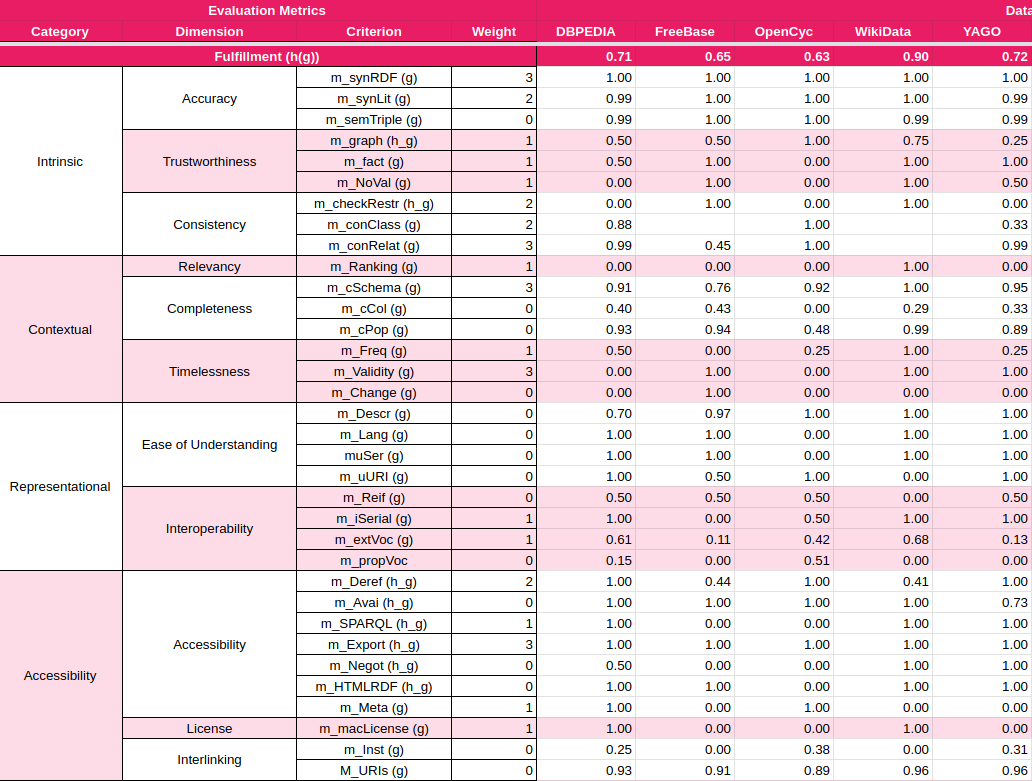
\includegraphics[scale=0.5]{content/appendix/figures/image.png}
\caption{Values for DBPEDIA, FreeBase, OpenCyc, WikiData and YAGO are taken from \cite{farber2017dataquality} as a rule. Exceptions are marked with '*' and explained in \autoref{app:kg_selection_framework}.
%Values for WordNet, ICEWS and GDELT are added \missing
}
\renewcommand{\arraystretch}{1.2}

\begin{comment}
\begin{tabular}{|m{2.5cm}|M|c|c|c|c|M|c|}
\hline
\thead{Method} & %method
\thead{Category} & %category
\thead{Temporal\\Information} & %temporal
\thead{Symmetric\\Relations} & %symmetry
\thead{Anti-\\Symmetric\\Relations} & %anti-symmetry
\thead{Entity\\Embedding} & %entity embedding
%\thead{Relation Embedding} & %relation embedding
\thead{Time\\Dimension} & %time dimension
\thead{Space} %space
\\
\hline
%\rowcolor{blue!10}
TransE \newline\cite{transe} & %method
Transformation \newline (translation) & %category
 & %temporal
 & %symmetry
\checkmark & %anti-symmetry
Separate & %entity embedding
%Single Vector & %relation embedding
\hrulefill & %time dimension
$\R$%space
\\
\hline
\end{tabular}
\end{comment}

\label{tab:selection_framework}
\end{minipage}
\end{table*}

Weights are assigned based on the perceived importance of a criterion relative to the project. They are determined as follows:
\begin{enumerate}
    \setcounter{enumi}{-1}
    \item Irrelevant
    \item Interesting, but most likely irrelevant
    \item Important
    \item Central
\end{enumerate}

In the following is given: a short description of each criterion; the assigned weight; reasoning behind the weight; notes where values have been changed from the original framework.

\subsection{Intrinsic Category}
The intrinsic category describes the data quality independent of the context.

\subsubsection{Accuracy}
The accuracy dimension describes whether the data is without errors.


\weighttable
{m_{synRDF(g)}}
{The syntactic validity of RDF documents.}
{3}
{Syntactic validity is necessary for machine interpretation and machine interpretation is necessary to train a model. As it is unrealistic to fix errors manually it is central that the documents are syntactically valid.}
{}

\weighttable
{m_{synLit}(g)}
{The syntactic validity of literals dependent on data types or pre-defined regular expressions.}
{2}
{The syntactic validity of literals is important as inconsistencies presumably affects the models negatively and we aim to analyze the models at their optimal performance. However it is possible to train the models and obtain a result even with syntactic invalidity in literals and as such it is not as important as $m_synRDF(g)$, the syntactic validity of documents.}
{The value for $m_{synLit}(YAGO)$ was changed from 0.62 to 0.99. The low value was due to YAGO allowing wildcards in the date datatype. As this is a feature in our context, the value was dismissed and an estimate was made based on the remaining factors.}

\weighttable
{m_{semTriple}(g)}
{The degree to which facts hold true.}
{0}
{The purpose of an embedding model is to represent available data and the performance of the model is evaluated against that same data. As such it is irrelevant whether the data holds true or not outside of the \gls{kg}.}
{}

\subsubsection{Trustworthiness}
The Trustworthiness dimension describes whether the data is credible.

\weighttable
{m_{graph}(h_g)}
{Trustworthiness on \gls{kg} level measured by manner of insertion and curation.}
{1}
{This criterion prioritizes manual over automatic work and experts over community. 
While we believe that this approach values the more reliable data higher and we acknowledge that the quality of training data highly impacts the quality of the resulting models, it is also noted that automatic means tend to yield bigger datasets, which also highly impacts the quality of the resulting models. Based on the assumption that significant problems will be revealed through other criteria we consider this criterion interesting, but likely irrelevant.}
{}

\weighttable
{m_{fact}(g)}
{Triples or documents are connected to sources}
{1}
{It lends credibility to the graph and is likely useful in a production setting, but while it is interesting, it is probably irrelevant as it is not the focus of the project and thus likely won't be of use.}
{}

\weighttable
{m_{NoVal}(g)}
{Indication of unknown and empty values}
{1}
{Could be used for negative sampling, as samples that are close to the truth are more valuable than those that are not \cite{yang2020negative-sampling, hyunh2019fact-checking-benchmark}. While this could help identification of those samples and negative sampling could improve model performance, it is not the focus of the project, probably won't be used and is thus interesting, but likely irrelevant.}
{The value for $m_{NoVal}(YAGO)$ was changed from 0 to 0.5 as YAGO does have some capacity for storing this information, through relations and use of wildcards to represent uncertainty.}

\subsubsection{Consistency}
The consistency dimension describes whether the data conflicts with itself.

\weighttable
{m_{checkRestr}(h_g)}
{Whether schema restrictions are checked at insertion time.}
{2}
{In general it is important that the data is consistent in order to enable models to properly represent the information.}
{}

\weighttable
{m_{conClass}(g)}
{Whether class restrictions are upheld.}
{2}
{It is important that class restrictions are upheld in order to eliminate possible sources of error, but as no hypothesis directly concerns class restrictions it is not central.}
{The values for $m_{conClass}(FreeBase)$ and $m_{conClass}(WikiData)$ are dismissed as the inspected constraints are not available in those graphs.}

\weighttable
{m_{conRelat}(g)}
{Whether relation restrictions are upheld.}
{3}
{As hypothesis \missing concerns model ability to represent various relations it is central that the relation constraints are upheld in the data.}
{The value for $m_{conClass}(WikiData)$ is dismissed as the inspected constraint is not available in that graph.}

\subsection{Contextual}
The contextual category describes the data quality in relation to the context.

\subsubsection{Relevancy}
The relevancy dimension describes whether the data is relevant to the purpose.

\weighttable
{m_{Ranking}(g)}
{Ranking of fact importance relative to one another}
{1}
{Could be used to extract more meaningful positive samples or when training models with an attention mechanism. However neither of those are the focus of this project and the information is thus interesting, but likely irrelevant.}
{The source is inconsistent in reports of $m_{Ranking}(FreeBase)$ and reports both 0 and 1. The 0 value is selected as it is consistent with the textual analysis and the values reported for remaining \glspl{kg}.}

\subsubsection{Completeness}
The completeness dimension describes whether the data is missing information relevant to the purpose.

\weighttable
{m_{cSchema}(g)}
{Quantifies missing classes and relations}
{3}
{As certain classes and relation are the subject of several analyses it is central that those classes and relations are present in the data. This is elaborated in \missing.}
{}

\weighttable
{m_{cCol}(g)}
{Quantifies missing relations on instances of classes}
{0}
{It is both an accepted reality and the point of the link prediction task that some information will be missing. While the total number of instances per relation is important, the degree to which entities are annotated with all entities is irrelevant.}
{}

\weighttable
{m_{cPop}(g)}
{Quantifies missing instances}
{0}
{This is irrelevant as the analysis concerns models' ability to embed data with certain characteristics rather than exact data.}
{}

\subsubsection{Timelessness}
The timelessness dimension describes whether the age af data is suitable for the purpose.

\weighttable
{m_{Freq}(g)}
{Frequency of updates}
{1}
{Data should be current to the extent that it is represented in current research to enable comparison of results and ease implementation efforts.}
{}

\weighttable
{m_{Validity}(g)}
{Specification of temporal validity}
{3}
{The project is focused on temporal embedding methods and as such the availability of temporal information is central to the analysis.}
{}

\weighttable
{m_{Change}(g)}
{Specification of last modification}
{0}
{In order to eliminate possible sources of error models are trained on static datasets and as such the modification date is irrelevant.}
{}

\subsection{Representational}
The representational category describes the format of data.

\subsubsection{Ease of Understanding}
The ease of understanding dimension describes whether the data is without ambiguity for a human.

\weighttable
{m_{Descr}(g)}
{Entities are labelled with descriptions.}
{0}
{The models do not need this information to train and the information is not valuable in the context of any hypotheses. As such it is irrelevant.}
{}

\weighttable
{m_{Lang}(g)}
{Contains labels in multiple languages}
{0}
{The models do not need this information to train and the information is not valuable in the context of any hypotheses. As such it is irrelevant.}
{}

\weighttable
{m_{uSer}(h_g)}
{More human-readable serialization formats are available.}
{0}
{The \gls{kg} used as input is not examined beyond its fulfillment of data quality requirements which are analyzed here. As such it is irrelevant whether it is human-readable or not.}
{}

\weighttable
{m_{uURI}(g)}
{Short, self-describing, non-generic URIs.}
{0}
{Though the value of immediately interpretable URIs to the human reader is obvious the value of clearly distinguishable URIs should not be dismissed and as the interpretation is available through labels the short URIs are irrelevant.}
{}

\subsubsection{Interoperability}
The interoperability dimension describes whether the data is without ambiguity for a computer.

\weighttable
{m_{Reif}(g)}
{Avoidance of blank nodes and reification statements.}
{0}
{The usage of blank nodes and reification statements could both improve and impair model performance. As it is not immediately obvious what impact their use has on model performance it is not possible to select the option allowing better model performance and as no hypothesis concerns this aspect whether they are used or not is irrelevant.}
{The source is inconsistent in its reports of $m_{Reif}(DBPEDIA)$ and reports both values of 0.5 and 1. The 0.5 value is selected as it is consistent with the textual analysis and the values reported for remaining \glspl{kg}.}

\weighttable
{m_{iSerial}(g)}
{The availability of other serialization formats.}
{1}
{Embedding methods typically require the input data in the format of tuples. While it is convenient to have the data supplied in the right format converting it is simple as long as it is syntactically valid and as such the availability of other formats is interesting, but likely irrelevant.}
{}

\weighttable
{m_{extVoc}(g)}
{Usage of external vocabulary for relations.}
{1}
{Multiple \glspl{kg} are analyzed in order to generalize observations. If all sources used the same vocabulary it would allow more fine-grained analysis and might simplify parts of the analysis, but the focus of our analysis is generally of a higher abstraction level and thus external vocabulary is interesting, but likely irrelevant.}
{The source is inconsistent in its reports of $m_{extVoc}(OpenCyc)$ and reports both values of 0.415 and 0.41. As this appears to be a rounding error the value 0.415 is used.}

\weighttable
{m_{propVoc}(g)}
{Linking the vocabulary to that of external sources.}
{0}
{In principle the reasoning is very similar to that of $m_{extVoc}(g)$. However this adds an additional layer of complexity to an already unlikely task, making the information irrelevant.}
{}

\subsection{Accessibility}
The accessibility category describes the accessibility of the data.

\subsubsection{Accessibility}
The accessibility dimension describes whether the data is available as well as the ease and speed of retrieval.

\weighttable
{m_{Deref}(h_g)}
{URIs are resolvable via HTTP requests.}
{2}
{It is important to have access to additional information about the resources in order to discover patterns.}
{The source has switched the values of $m_{Deref}(h_{FreeBase})$ and $m_{Deref}(h_{OpenCyc})$ in at least one instance. $m_{Deref}(h_{FreeBase})$ is set to 0.437 and $m_{Deref}(h_{OpenCyc})$ is set to 1 as those are the most commonly reported numbers and consistent with the textual analysis.}

\weighttable
{m_{Avai}(h_g)}
{Uptime of the \gls{kg}.}
{0}
{As only static data is queried it is irrelevant.}
{The source has switched the values of $m_{Avai}(h_{FreeBase})$ and $m_{Avai}(h_{YAGO})$ in at least one instance. $m_{Avai}(h_{FreeBase})$ is set to 0.9998 and $m_{Avai}(h_{YAGO})$ is set to 0.7306 as those are the most commonly reported numbers and consistent with the textual analysis.}

\weighttable
{m_{SPARQL}(h_g)}
{The availability of a SPARQL endpoint.}
{1}
{In a production setting this would likely be necessary, but as that is outside the scope of this project it is interesting, but likely irrelevant.}
{The source has switched the values of $m_{SPARQL}(h_{FreeBase})$ and $m_{SPARQL}(h_{YAGO})$ in at least one instance. $m_{SPARQL}(h_{FreeBase})$ is set to 0 and $m_{SPAQRL}(h_{YAGO})$ is set to 1 as those are the most commonly reported numbers and consistent with the textual analysis.}

\weighttable
{m_{Export}(h_g)}
{The ability to export the data in RDF format.}
{3}
{In order to eliminate possible sources of error models are trained on static datasets which are exported from the \gls{kg} and the ability to so is therefore central.}
{}

\weighttable
{m_{Negot}(h_g)}
{Support of content negotiation that is dereferencing sources in client's preferred serialization format.}
{0}
{As long as content is returned in a valid serialization format the exact format is largely irrelevant.}
{The source has switched the values of $m_{Negot}(h_{FreeBase})$ and $m_{Negot}(h_{YAGO})$ in at least one instance. $m_{Negot}(h_{FreeBase})$ is set to 0 and $m_{Negot}(h_{YAGO})$ is set to 1 as those are the most commonly reported numbers and consistent with the textual analysis.}

\weighttable
{m_{HTMLRDF}(h_g)}
{Linking HTML descriptions and RDF serializations to facilitate automatic link discovery.}
{0}
{While possibly useful to improve the performance of embedding models, we are unaware of any embedding methods utilizing it and it is therefore irrelevant.}
{The source has switched the values of $m_{HTMLRDF}(h_{OpenCyc})$ and $m_{HTMLRDF}(h_{YAGO})$ in at least one instance. $m_{HTMLRDF}(h_{OpenCyc})$ is set to 0 and $m_{HTMLRDF}(h_{YAGO})$ is set to 1 as those are the most commonly reported numbers and consistent with the textual analysis.}

\weighttable
{m_{Meta}(g)}
{Machine-readable metadata via sitemaps and VoID.}
{1}
{Some embedding methods make use of metadata to improve the performance of the model. As this aspect is not covered in any hypothesis, the information is interesting, but likely irrelevant.}
{The source has switched the values of $m_{Meta}(OpenCyc)$ and $m_{Meta}(YAGO)$ in at least one instance. $m_{Meta}(OpenCyc)$ is set to 1 and $m_{Meta}(YAGO)$ is set to 0 as those are the most commonly reported numbers and consistent with the textual analysis.}

\subsubsection{License}
The license dimension describes the license the data is subject to.

\weighttable
{m_{macLicense}(g)}
{Availability of machine-readable license.}
{1}
{It is important that there is a license permitting our use of the data but as a human-readable version is sufficient it is interesting, but likely irrelevant whether a machine-readable one exists.}
{}

\subsubsection{Interlinking}
The interlinking dimension describes whether data representing the same entities is linked.

\weighttable
{m_{Inst}(g)}
{Equivalence links to external sources.}
{0}
{This would only be relevant if models were trained on combined graphs. As that is not the case it is irrelevant.}
{The source is inconsistent in its reports of $m_{Inst}(DBPEDIA)$ and $m_{Inst}(OpenCyc)$. $m_{Inst}(DBPEDIA)$ is reported as 0.592 and 0.251 and $m_{Inst}(OpenCyc)$ is reported as 0.443 and 0.382.
$m_{Inst}(DBPEDIA)$ is set to 0.251 and $m_{Inst}(OpenCyc)$ is set to 0.382 as those are the most commonly reported numbers and consistent with the textual analysis.}

\weighttable
{m_{URI}(g)}
{Validity of of external URIs.}
{0}
{This is irrelevant as the external URIs are not used.}
{The source is inconsistent in its reports of $m_{URI}(DBPEDIA)$ and $m_{URI}(FreeBase)$ and the textual analysis does not resolve these inconsistencies. $m_{URI}(DBPEDIA)$ is set to 0.929 and $m_{URI}(FreeBase)$ is set to 0.908 as those are the most common values. It is also noted that greatest value difference is 0.06.}
\endgroup
\section{Time Prediction Error Distribution}
\label{time_prediction_error_distribution}

 \begin{figure}[htb]
\centering
\begin{minipage}{0.95\columnwidth}
\centering
\begin{tikzpicture}
\begin{axis}[
no markers,
xlabel={Error},
ylabel={\# Occurences}]

\addplot table {content/appendix/figures/time_prediction_distribution/error_distribution_DE_TransE_icews14_diff.dat};

\end{axis}
\end{tikzpicture}
\vspace{-3mm}
\caption{Distribution of predictions on timestamps for DE\_TransE on icews14}
\label{fig:time_prediction_distribution_DE_TransE_icews14}
\end{minipage}
\end{figure}
 \begin{figure}[htb]
\centering
\begin{minipage}{0.95\columnwidth}
\centering
\begin{tikzpicture}
\begin{axis}[
no markers,
xlabel={Error},
ylabel={\# Occurences}]

\addplot table {content/appendix/figures/time_prediction_distribution/error_distribution_DE_SimplE_icews14_diff.dat};

\end{axis}
\end{tikzpicture}
\vspace{-3mm}
\caption{Distribution of predictions on timestamps for DE\_SimplE on icews14}
\label{fig:time_prediction_distribution_DE_SimplE_icews14}
\end{minipage}
\end{figure}
 \begin{figure}[htb]
\centering
\begin{minipage}{0.95\columnwidth}
\centering
\begin{tikzpicture}
\begin{axis}[
no markers,
xlabel={Error},
ylabel={\# Occurences}]

\addplot table {content/appendix/figures/time_prediction_distribution/error_distribution_DE_DistMult_icews14_diff.dat};

\end{axis}
\end{tikzpicture}
\vspace{-3mm}
\caption{Distribution of predictions on timestamps for DE\_DistMult on icews14}
\label{fig:time_prediction_distribution_DE_DistMult_icews14}
\end{minipage}
\end{figure}
 \begin{figure}[htb]
\centering
\begin{minipage}{0.95\columnwidth}
\centering
\begin{tikzpicture}
\begin{axis}[
no markers,
xlabel={Error},
ylabel={\# Occurences}]

\addplot table {content/appendix/figures/time_prediction_distribution/error_distribution_TERO_icews14_diff.dat};

\end{axis}
\end{tikzpicture}
\vspace{-3mm}
\caption{Distribution of predictions on timestamps for TERO on icews14}
\label{fig:time_prediction_distribution_TERO_icews14}
\end{minipage}
\end{figure}
 \begin{figure}[htb]
\centering
\begin{minipage}{0.95\columnwidth}
\centering
\begin{tikzpicture}
\begin{axis}[
no markers,
xlabel={Error},
ylabel={\# Occurences}]

\addplot table {content/appendix/figures/time_prediction_distribution/error_distribution_ATISE_icews14_diff.dat};

\end{axis}
\end{tikzpicture}
\vspace{-3mm}
\caption{Distribution of predictions on timestamps for ATISE on icews14}
\label{fig:time_prediction_distribution_ATISE_icews14}
\end{minipage}
\end{figure}
\begin{figure}[htb]
\centering
\begin{minipage}{0.95\columnwidth}
\centering
\begin{tikzpicture}
\begin{axis}[
no markers,
xlabel={Error},
ylabel={\# Occurences}]

\addplot table {content/appendix/figures/time_prediction_distribution/error_distribution_DE_TransE_wikidata12k_diff.dat};

\end{axis}
\end{tikzpicture}
\vspace{-3mm}
\caption{Distribution of predictions on timestamps for DE\_TransE on wikidata12k}
\label{fig:time_prediction_distribution_DE_TransE_wikidata12k}
\end{minipage}
\end{figure}
\begin{figure}[htb]
\centering
\begin{minipage}{0.95\columnwidth}
\centering
\begin{tikzpicture}
\begin{axis}[
no markers,
xlabel={Error},
ylabel={\# Occurences}]

\addplot table {content/appendix/figures/time_prediction_distribution/error_distribution_DE_SimplE_wikidata12k_diff.dat};

\end{axis}
\end{tikzpicture}
\vspace{-3mm}
\caption{Distribution of predictions on timestamps for DE\_SimplE on wikidata12k}
\label{fig:time_prediction_distribution_DE_SimplE_wikidata12k}
\end{minipage}
\end{figure}
\begin{figure}[htb]
\centering
\begin{minipage}{0.95\columnwidth}
\centering
\begin{tikzpicture}
\begin{axis}[
no markers,
xlabel={Error},
ylabel={\# Occurences}]

\addplot table {content/appendix/figures/time_prediction_distribution/error_distribution_DE_DistMult_wikidata12k_diff.dat};

\end{axis}
\end{tikzpicture}
\vspace{-3mm}
\caption{Distribution of predictions on timestamps for DE\_DistMult on wikidata12k}
\label{fig:time_prediction_distribution_DE_DistMult_wikidata12k}
\end{minipage}
\end{figure}
\begin{figure}[htb]
\centering
\begin{minipage}{0.95\columnwidth}
\centering
\begin{tikzpicture}
\begin{axis}[
no markers,
xlabel={Error},
ylabel={\# Occurences}]

\addplot table {content/appendix/figures/time_prediction_distribution/error_distribution_TERO_wikidata12k_best.dat};

\end{axis}
\end{tikzpicture}
\vspace{-3mm}
\caption{Distribution of best case predictions on timestamps for TERO on wikidata12k}
\label{fig:time_prediction_distribution_TERO_wikidata12k_best}
\end{minipage}
\end{figure}
\begin{figure}[htb]
\centering
\begin{minipage}{0.95\columnwidth}
\centering
\begin{tikzpicture}
\begin{axis}[
no markers,
xlabel={Error},
ylabel={\# Occurences}]

\addplot table {content/appendix/figures/time_prediction_distribution/error_distribution_TERO_wikidata12k_wors.dat};

\end{axis}
\end{tikzpicture}
\vspace{-3mm}
\caption{Distribution of worst case predictions on timestamps for TERO on wikidata12k}
\label{fig:time_prediction_distribution_TERO_wikidata12k_wors}
\end{minipage}
\end{figure}
\begin{figure}[htb]
\centering
\begin{minipage}{0.95\columnwidth}
\centering
\begin{tikzpicture}
\begin{axis}[
no markers,
xlabel={Error},
ylabel={\# Occurences}]

\addplot table {content/appendix/figures/time_prediction_distribution/error_distribution_ATISE_wikidata12k_best.dat};

\end{axis}
\end{tikzpicture}
\vspace{-3mm}
\caption{Distribution of best case predictions on timestamps for ATISE on wikidata12k}
\label{fig:time_prediction_distribution_ATISE_wikidata12k_best}
\end{minipage}
\end{figure}
\begin{figure}[htb]
\centering
\begin{minipage}{0.95\columnwidth}
\centering
\begin{tikzpicture}
\begin{axis}[
no markers,
xlabel={Error},
ylabel={\# Occurences}]

\addplot table {content/appendix/figures/time_prediction_distribution/error_distribution_ATISE_wikidata12k_wors.dat};

\end{axis}
\end{tikzpicture}
\vspace{-3mm}
\caption{Distribution of worst case predictions on timestamps for ATISE on wikidata12k}
\label{fig:time_prediction_distribution_ATISE_wikidata12k_wors}
\end{minipage}
\end{figure}
\begin{figure}[htb]
\centering
\begin{minipage}{0.95\columnwidth}
\centering
\begin{tikzpicture}
\begin{axis}[
no markers,
xlabel={Error},
ylabel={\# Occurences}]

\addplot table {content/appendix/figures/time_prediction_distribution/error_distribution_DE_TransE_yago11k_diff.dat};

\end{axis}
\end{tikzpicture}
\vspace{-3mm}
\caption{Distribution of predictions on timestamps for DE\_TransE on yago11k}
\label{fig:time_prediction_distribution_DE_TransE_yago11k}
\end{minipage}
\end{figure}
\begin{figure}[htb]
\centering
\begin{minipage}{0.95\columnwidth}
\centering
\begin{tikzpicture}
\begin{axis}[
no markers,
xlabel={Error},
ylabel={\# Occurences}]

\addplot table {content/appendix/figures/time_prediction_distribution/error_distribution_DE_SimplE_yago11k_diff.dat};

\end{axis}
\end{tikzpicture}
\vspace{-3mm}
\caption{Distribution of predictions on timestamps for DE\_SimplE on yago11k}
\label{fig:time_prediction_distribution_DE_SimplE_yago11k}
\end{minipage}
\end{figure}
\begin{figure}[htb]
\centering
\begin{minipage}{0.95\columnwidth}
\centering
\begin{tikzpicture}
\begin{axis}[
no markers,
xlabel={Error},
ylabel={\# Occurences}]

\addplot table {content/appendix/figures/time_prediction_distribution/error_distribution_DE_DistMult_yago11k_diff.dat};

\end{axis}
\end{tikzpicture}
\vspace{-3mm}
\caption{Distribution of predictions on timestamps for DE\_DistMult on yago11k}
\label{fig:time_prediction_distribution_DE_DistMult_yago11k}
\end{minipage}
\end{figure}
\begin{figure}[htb]
\centering
\begin{minipage}{0.95\columnwidth}
\centering
\begin{tikzpicture}
\begin{axis}[
no markers,
xlabel={Error},
ylabel={\# Occurences}]

\addplot table {content/appendix/figures/time_prediction_distribution/error_distribution_TERO_yago11k_best.dat};

\end{axis}
\end{tikzpicture}
\vspace{-3mm}
\caption{Distribution of predictions on timestamps for TERO on yago11k}
\label{fig:time_prediction_distribution_TERO_yago11k_best}
\end{minipage}
\end{figure}
\begin{figure}[htb]
\centering
\begin{minipage}{0.95\columnwidth}
\centering
\begin{tikzpicture}
\begin{axis}[
no markers,
xlabel={Error},
ylabel={\# Occurences}]

\addplot table {content/appendix/figures/time_prediction_distribution/error_distribution_TERO_yago11k_wors.dat};

\end{axis}
\end{tikzpicture}
\vspace{-3mm}
\caption{Distribution of worst case predictions on timestamps for TERO on yago11k}
\label{fig:time_prediction_distribution_TERO_yago11k_wors}
\end{minipage}
\end{figure}
\begin{figure}[htb]
\centering
\begin{minipage}{0.95\columnwidth}
\centering
\begin{tikzpicture}
\begin{axis}[
no markers,
xlabel={Error},
ylabel={\# Occurences}]

\addplot table {content/appendix/figures/time_prediction_distribution/error_distribution_ATISE_yago11k_best.dat};

\end{axis}
\end{tikzpicture}
\vspace{-3mm}
\caption{Distribution of best case predictions on timestamps for ATISE on yago11k}
\label{fig:time_prediction_distribution_ATISE_yago11k_best}
\end{minipage}
\end{figure}
\begin{figure}[htb]
\centering
\begin{minipage}{0.95\columnwidth}
\centering
\begin{tikzpicture}
\begin{axis}[
no markers,
xlabel={Error},
ylabel={\# Occurences}]

\addplot table {content/appendix/figures/time_prediction_distribution/error_distribution_ATISE_yago11k_wors.dat};

\end{axis}
\end{tikzpicture}
\vspace{-3mm}
\caption{Distribution of worst case predictions on timestamps for ATISE on yago11k}
\label{fig:time_prediction_distribution_ATISE_yago11k_wors}
\end{minipage}
\end{figure}

\clearpage
\onecolumn
\section{Comparisons between datasets and splits}
\label{app:dataset_split_comparisons}

\begin{figure*}[ht]
\centering
\begin{minipage}{0.9\textwidth}
\centering
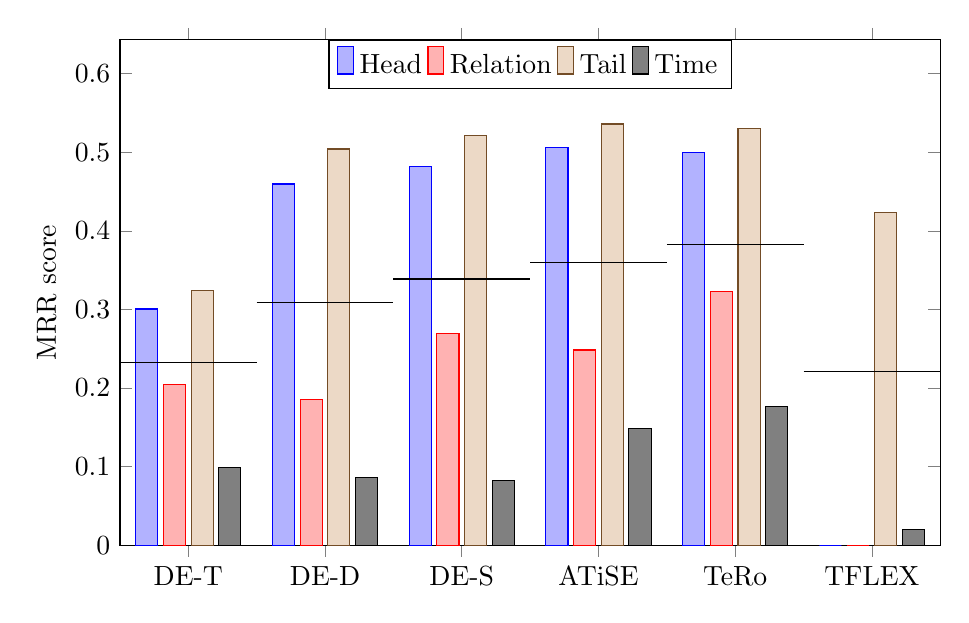
\begin{tikzpicture}
\begin{axis}[
    ybar,
    bar width=8pt,
    xticklabels={x,DE-T,DE-D,DE-S,ATiSE,TeRo,TFLEX},
    ymin=0,
    ymax=0.6431143840995598,
    ylabel={MRR score},
    height=8cm,
    width=12cm,
    legend style={
        at={(0.5,1.0)},
        anchor=north,
        legend columns=-1
    },
    legend image code/.code={
        \draw [#1] (0cm,-0.1cm) rectangle (0.2cm,0.25cm); },
    ]
\addplot coordinates { %head
(0, 0.30052498907664305) %DE_TransE
(1, 0.4595339060848753) %DE_DistMult
(2, 0.48168727741357964) %DE_SimplE
(3, 0.5054803290523) %ATISE
(4, 0.5000763027042784) %TERO
(5, 0) %TFLEX
} ;
\addplot coordinates { %relation
(0, 0.204748279197774) %DE_TransE
(1, 0.18564274192135086) %DE_DistMult
(2, 0.26905439575244017) %DE_SimplE
(3, 0.24829059776365678) %ATISE
(4, 0.32241041307968443) %TERO
(5, 0) %TFLEX
} ;
\addplot coordinates { %tail
(0, 0.3235768065354983) %DE_TransE
(1, 0.5041639225422816) %DE_DistMult
(2, 0.5215051513802474) %DE_SimplE
(3, 0.5359286534162998) %ATISE
(4, 0.5302146473852904) %TERO
(5, 0.4230984270644139) %TFLEX
} ;
\addplot coordinates { %time_from
(0, 0.09877310207544412) %DE_TransE
(1, 0.0861250207110118) %DE_DistMult
(2, 0.08222193019657349) %DE_SimplE
(3, 0.1488256559822522) %ATISE
(4, 0.17619341931881538) %TERO
(5, 0.019646307923523638) %TFLEX
} ;
\addplot[black,sharp plot,update limits=false,] coordinates { %DE_TransE
(-0.5, 0.23190579422133198)
(0.5, 0.23190579422133198)
} ;
\addplot[black,sharp plot,update limits=false,] coordinates { %DE_DistMult
(0.5, 0.30886639781489195)
(1.5, 0.30886639781489195)
} ;
\addplot[black,sharp plot,update limits=false,] coordinates { %DE_SimplE
(1.5, 0.33861718868573143)
(2.5, 0.33861718868573143)
} ;
\addplot[black,sharp plot,update limits=false,] coordinates { %ATISE
(2.5, 0.3596313090536477)
(3.5, 0.3596313090536477)
} ;
\addplot[black,sharp plot,update limits=false,] coordinates { %TERO
(3.5, 0.382223695622041)
(4.5, 0.382223695622041)
} ;
\addplot[black,sharp plot,update limits=false,] coordinates { %TFLEX
(4.5, 0.22137236749396744)
(5.5, 0.22137236749396744)
} ;
\legend{Head,Relation,Tail,Time}
\end{axis}
\end{tikzpicture}
\caption{icews14, split original}
\label{fig:compare_icews14_original}
\end{minipage}
\end{figure*}

%\begin{figure*}[ht]
\centering
\begin{minipage}{0.9\textwidth}
\centering
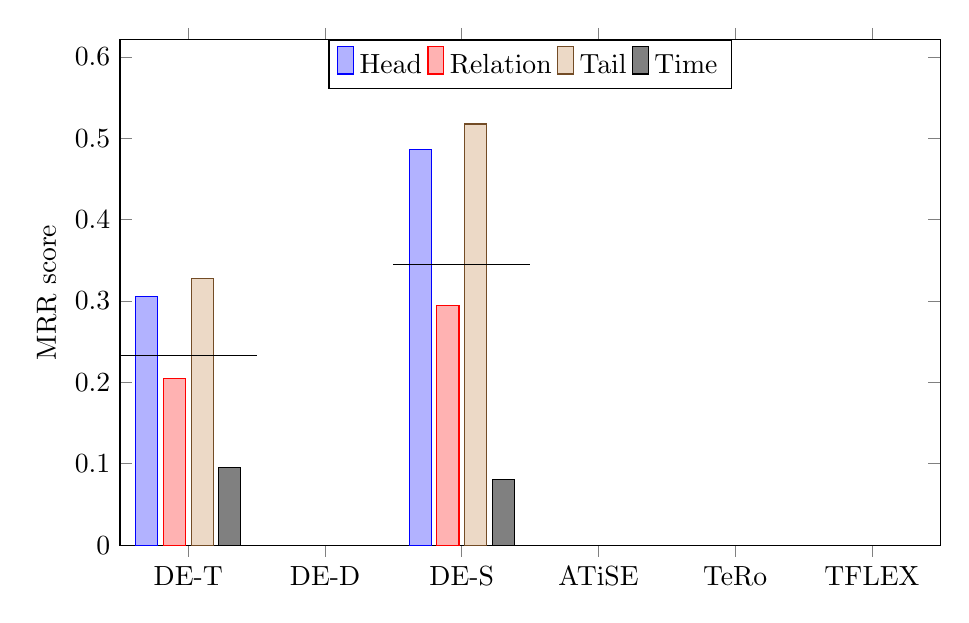
\begin{tikzpicture}
\begin{axis}[
    ybar,
    bar width=8pt,
    xticklabels={x,DE-T,DE-D,DE-S,ATiSE,TeRo,TFLEX},
    ymin=0,
    ymax=0.6209152961250467,
    ylabel={MRR score},
    height=8cm,
    width=12cm,
    legend style={
        at={(0.5,1.0)},
        anchor=north,
        legend columns=-1
    },
    legend image code/.code={
        \draw [#1] (0cm,-0.1cm) rectangle (0.2cm,0.25cm); },
    ]
\addplot coordinates { %head
(0, 0.3060130826437023) %DE_TransE
(1, 0) %DE_DistMult
(2, 0.485840495935422) %DE_SimplE
(3, 0) %ATISE
(4, 0) %TERO
(5, 0) %TFLEX
} ;
\addplot coordinates { %relation
(0, 0.2050733839712357) %DE_TransE
(1, 0) %DE_DistMult
(2, 0.29419180983873955) %DE_SimplE
(3, 0) %ATISE
(4, 0) %TERO
(5, 0) %TFLEX
} ;
\addplot coordinates { %tail
(0, 0.3277892854794874) %DE_TransE
(1, 0) %DE_DistMult
(2, 0.5174294134375389) %DE_SimplE
(3, 0) %ATISE
(4, 0) %TERO
(5, 0) %TFLEX
} ;
\addplot coordinates { %time_from
(0, 0.09517766038307589) %DE_TransE
(1, 0) %DE_DistMult
(2, 0.0809454461243896) %DE_SimplE
(3, 0) %ATISE
(4, 0) %TERO
(5, 0) %TFLEX
} ;
\addplot[black,sharp plot,update limits=false,] coordinates { %DE_TransE
(-0.5, 0.23351335311939853)
(0.5, 0.23351335311939853)
} ;
\addplot[black,sharp plot,update limits=false,] coordinates { %DE_DistMult
(0.5, 0)
(1.5, 0)
} ;
\addplot[black,sharp plot,update limits=false,] coordinates { %DE_SimplE
(1.5, 0.3446017913340443)
(2.5, 0.3446017913340443)
} ;
\addplot[black,sharp plot,update limits=false,] coordinates { %ATISE
(2.5, 0)
(3.5, 0)
} ;
\addplot[black,sharp plot,update limits=false,] coordinates { %TERO
(3.5, 0)
(4.5, 0)
} ;
\addplot[black,sharp plot,update limits=false,] coordinates { %TFLEX
(4.5, 0)
(5.5, 0)
} ;
\legend{Head,Relation,Tail,Time}
\end{axis}
\end{tikzpicture}
\caption{icews14, split 1}
\label{fig:compare_icews14_1}
\end{minipage}
\end{figure*}

%\begin{figure}[htb]
\centering
\begin{minipage}{\columnwidthcaption}
\resizebox{\columnwidthcaption}{!}{
\centering
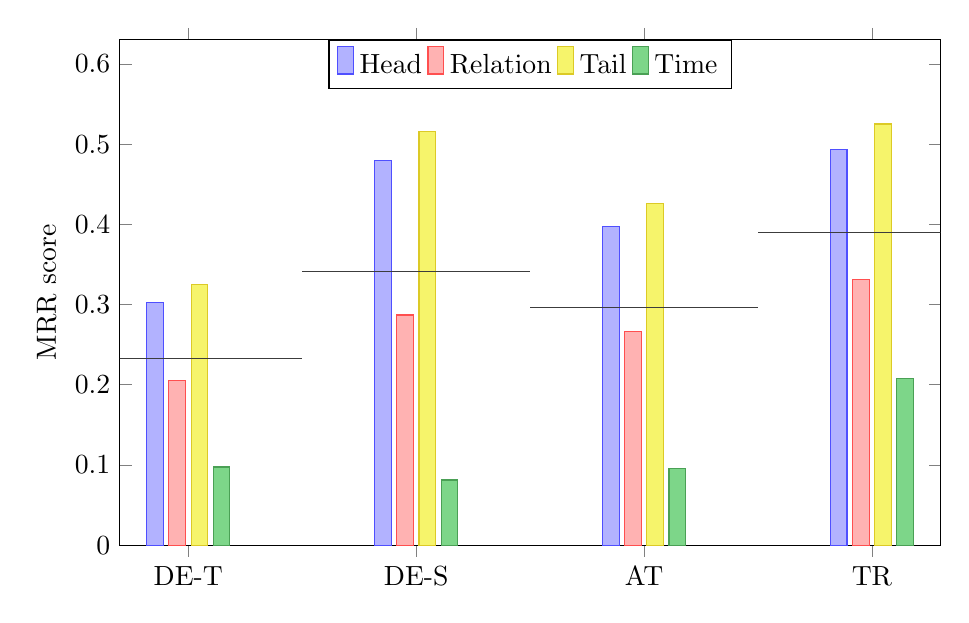
\begin{tikzpicture}
\begin{axis}[
    ybar,
    bar width=6pt,
    xtick={0,1,2,3},
    xticklabels={DE-T,DE-S,AT,TR},
    ymin=0,
    ymax=0.6302926133299789,
    ylabel={MRR score},
    height=8cm,
    width=12cm,
    legend style={
        at={(0.5,1.0)},
        anchor=north,
        legend columns=-1
    },
    legend image code/.code={
        \draw [#1] (0cm,-0.1cm) rectangle (0.2cm,0.25cm); },
    ]
\addplot[color=ourdarkblue, fill=ourlightblue] coordinates { %head
(0, 0.30216451910382897) %DE_TransE
(1, 0.47975397629017363) %DE_SimplE
(2, 0.39751251243884284) %ATISE
(3, 0.4932383272431821) %TERO
} ;
\addplot[color=ourdarkred, fill=ourlightred] coordinates { %relation
(0, 0.20561360677141266) %DE_TransE
(1, 0.2870517171097706) %DE_SimplE
(2, 0.2659269486815848) %ATISE
(3, 0.33087666516359965) %TERO
} ;
\addplot[color=ourdarkyellow, fill=ourlightyellow] coordinates { %tail
(0, 0.32552183746961566) %DE_TransE
(1, 0.5155838483952053) %DE_SimplE
(2, 0.42563392854801446) %ATISE
(3, 0.5252438444416491) %TERO
} ;
\addplot[color=ourdarkgreen, fill=ourlightgreen] coordinates { %time_from
(0, 0.097430832145382) %DE_TransE
(1, 0.08117405573647266) %DE_SimplE
(2, 0.09575877501848301) %ATISE
(3, 0.20822111118193068) %TERO
} ;
\addplot[ourblack,sharp plot,update limits=false,] coordinates { %DE_TransE
(-0.5, 0.23268269887258053)
(0.5, 0.23268269887258053)
} ;
\addplot[ourblack,sharp plot,update limits=false,] coordinates { %DE_SimplE
(0.5, 0.3408908993829318)
(1.5, 0.3408908993829318)
} ;
\addplot[ourblack,sharp plot,update limits=false,] coordinates { %ATISE
(1.5, 0.2962080411717723)
(2.5, 0.2962080411717723)
} ;
\addplot[ourblack,sharp plot,update limits=false,] coordinates { %TERO
(2.5, 0.38939498700761177)
(3.5, 0.38939498700761177)
} ;
\legend{Head,Relation,Tail,Time}
\end{axis}
\end{tikzpicture}
}
\caption{ICEWS, split 2}
\label{fig:compare_icews14_2}
\end{minipage}
\end{figure}

%\begin{figure*}[ht]
\centering
\begin{minipage}{0.9\textwidth}
\centering
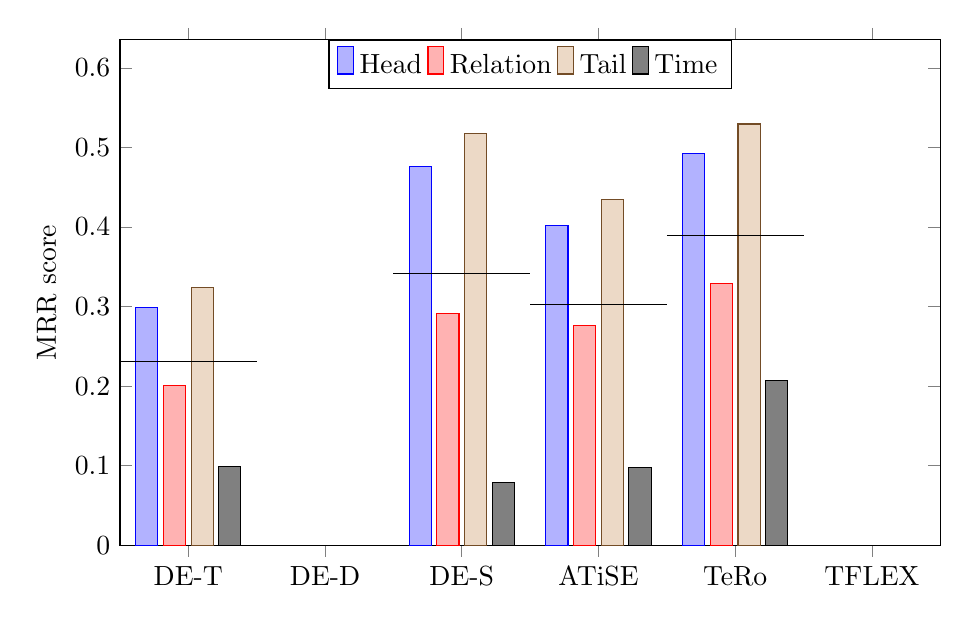
\begin{tikzpicture}
\begin{axis}[
    ybar,
    bar width=8pt,
    xticklabels={x,DE-T,DE-D,DE-S,ATiSE,TeRo,TFLEX},
    ymin=0,
    ymax=0.6354346838209075,
    ylabel={MRR score},
    height=8cm,
    width=12cm,
    legend style={
        at={(0.5,1.0)},
        anchor=north,
        legend columns=-1
    },
    legend image code/.code={
        \draw [#1] (0cm,-0.1cm) rectangle (0.2cm,0.25cm); },
    ]
\addplot coordinates { %head
(0, 0.29844506503622253) %DE_TransE
(1, 0) %DE_DistMult
(2, 0.4765422096798048) %DE_SimplE
(3, 0.40172910580674936) %ATISE
(4, 0.4919566468517329) %TERO
(5, 0) %TFLEX
} ;
\addplot coordinates { %relation
(0, 0.20077569619293) %DE_TransE
(1, 0) %DE_DistMult
(2, 0.2912021752094241) %DE_SimplE
(3, 0.27662462973329455) %ATISE
(4, 0.3294132165208661) %TERO
(5, 0) %TFLEX
} ;
\addplot coordinates { %tail
(0, 0.32347901873329166) %DE_TransE
(1, 0) %DE_DistMult
(2, 0.517960822980905) %DE_SimplE
(3, 0.43475112043661623) %ATISE
(4, 0.5295289031840896) %TERO
(5, 0) %TFLEX
} ;
\addplot coordinates { %time_from
(0, 0.09900230537341467) %DE_TransE
(1, 0) %DE_DistMult
(2, 0.07828203173373395) %DE_SimplE
(3, 0.09790601285764011) %ATISE
(4, 0.20690000739430325) %TERO
(5, 0) %TFLEX
} ;
\addplot[black,sharp plot,update limits=false,] coordinates { %DE_TransE
(-0.5, 0.23042552133398808)
(0.5, 0.23042552133398808)
} ;
\addplot[black,sharp plot,update limits=false,] coordinates { %DE_DistMult
(0.5, 0)
(1.5, 0)
} ;
\addplot[black,sharp plot,update limits=false,] coordinates { %DE_SimplE
(1.5, 0.3409968099009897)
(2.5, 0.3409968099009897)
} ;
\addplot[black,sharp plot,update limits=false,] coordinates { %ATISE
(2.5, 0.30275271720861785)
(3.5, 0.30275271720861785)
} ;
\addplot[black,sharp plot,update limits=false,] coordinates { %TERO
(3.5, 0.3894496934877669)
(4.5, 0.3894496934877669)
} ;
\addplot[black,sharp plot,update limits=false,] coordinates { %TFLEX
(4.5, 0)
(5.5, 0)
} ;
\legend{Head,Relation,Tail,Time}
\end{axis}
\end{tikzpicture}
\caption{icews14, split 3}
\label{fig:compare_icews14_3}
\end{minipage}
\end{figure*}

%\clearpage
\begin{figure*}[ht]
\centering
\begin{minipage}{0.9\textwidth}
\centering
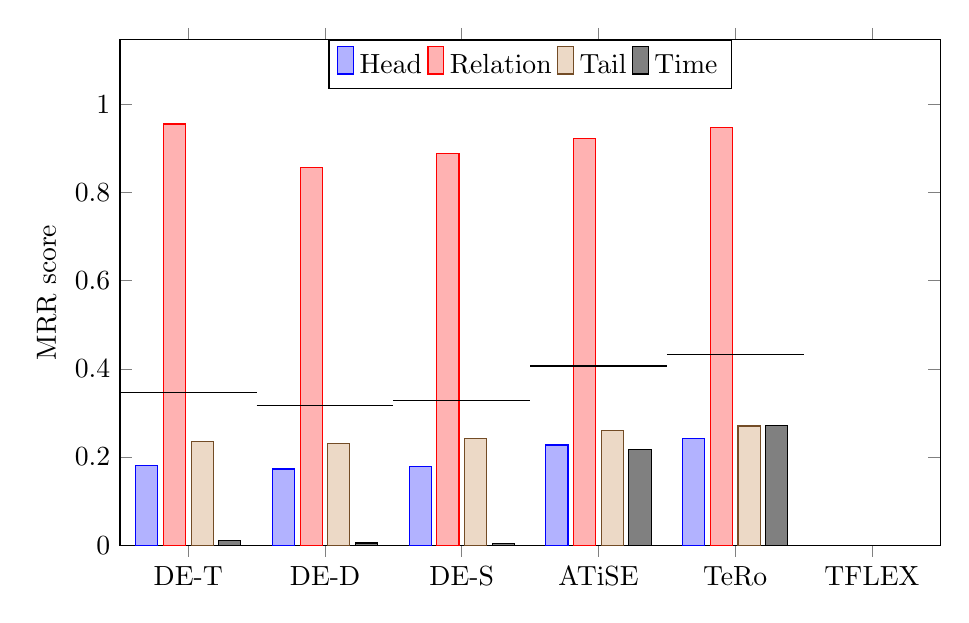
\begin{tikzpicture}
\begin{axis}[
    ybar,
    bar width=8pt,
    xticklabels={x,DE-T,DE-D,DE-S,ATiSE,TeRo,TFLEX},
    ymin=0,
    ymax=1.1469754572524147,
    ylabel={MRR score},
    height=8cm,
    width=12cm,
    legend style={
        at={(0.5,1.0)},
        anchor=north,
        legend columns=-1
    },
    legend image code/.code={
        \draw [#1] (0cm,-0.1cm) rectangle (0.2cm,0.25cm); },
    ]
\addplot coordinates { %head
(0, 0.18130037449949188) %DE_TransE
(1, 0.17282233690181947) %DE_DistMult
(2, 0.1780547872213373) %DE_SimplE
(3, 0.2273298150215758) %ATISE
(4, 0.24186633018673434) %TERO
(5, 0) %TFLEX
} ;
\addplot coordinates { %relation
(0, 0.9558128810436789) %DE_TransE
(1, 0.8572876609776997) %DE_DistMult
(2, 0.8880839024104603) %DE_SimplE
(3, 0.922117713779801) %ATISE
(4, 0.9472559198556247) %TERO
(5, 0) %TFLEX
} ;
\addplot coordinates { %tail
(0, 0.235634963095345) %DE_TransE
(1, 0.23166552322567083) %DE_DistMult
(2, 0.24154788434002833) %DE_SimplE
(3, 0.2591914088614538) %ATISE
(4, 0.2704648943835616) %TERO
(5, 0) %TFLEX
} ;
\addplot coordinates { %time_from
(0, 0.010488972252275434) %DE_TransE
(1, 0.004897539365177376) %DE_DistMult
(2, 0.004360166639279628) %DE_SimplE
(3, 0.21756454450370288) %ATISE
(4, 0.2706700220390521) %TERO
(5, 0) %TFLEX
} ;
\addplot[black,sharp plot,update limits=false,] coordinates { %DE_TransE
(-0.5, 0.3458092977226949)
(0.5, 0.3458092977226949)
} ;
\addplot[black,sharp plot,update limits=false,] coordinates { %DE_DistMult
(0.5, 0.31666826511758944)
(1.5, 0.31666826511758944)
} ;
\addplot[black,sharp plot,update limits=false,] coordinates { %DE_SimplE
(1.5, 0.3280116851527744)
(2.5, 0.3280116851527744)
} ;
\addplot[black,sharp plot,update limits=false,] coordinates { %ATISE
(2.5, 0.40655087054162753)
(3.5, 0.40655087054162753)
} ;
\addplot[black,sharp plot,update limits=false,] coordinates { %TERO
(3.5, 0.43256429161623894)
(4.5, 0.43256429161623894)
} ;
\addplot[black,sharp plot,update limits=false,] coordinates { %TFLEX
(4.5, 0)
(5.5, 0)
} ;
\legend{Head,Relation,Tail,Time}
\end{axis}
\end{tikzpicture}
\caption{wikidata12k, split original}
\label{fig:compare_wikidata12k_original}
\end{minipage}
\end{figure*}

%\begin{figure}[htb]
\centering
\begin{minipage}{\columnwidthcaption}
\resizebox{\columnwidthcaption}{!}{
\centering
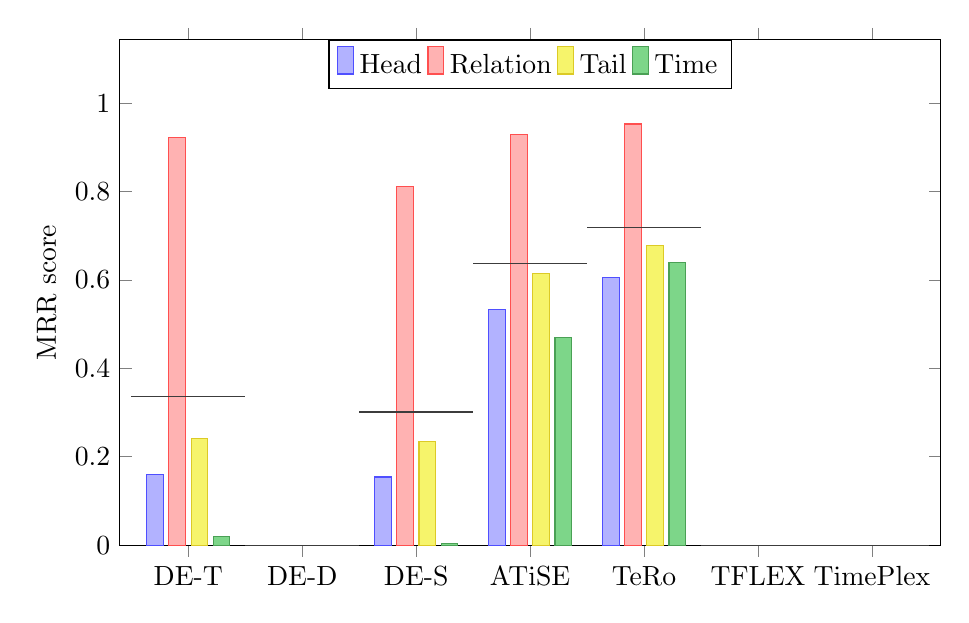
\begin{tikzpicture}
\begin{axis}[
    ybar,
    bar width=6pt,
    xticklabels={x,DE-T,DE-D,DE-S,ATiSE,TeRo,TFLEX,TimePlex},
    ymin=0,
    ymax=1.1435875200261874,
    ylabel={MRR score},
    height=8cm,
    width=12cm,
    legend style={
        at={(0.5,1.0)},
        anchor=north,
        legend columns=-1
    },
    legend image code/.code={
        \draw [#1] (0cm,-0.1cm) rectangle (0.2cm,0.25cm); },
    ]
\addplot[color=ourdarkblue, fill=ourlightblue] coordinates { %head
(0, 0.1600322415080232) %DE_TransE
(1, 0) %DE_DistMult
(2, 0.15417392324803428) %DE_SimplE
(3, 0.5337434445473753) %ATISE
(4, 0.6058347902914908) %TERO
(5, 0) %TFLEX
(6, 0) %TimePlex
} ;
\addplot[color=ourdarkred, fill=ourlightred] coordinates { %relation
(0, 0.9218881599136685) %DE_TransE
(1, 0) %DE_DistMult
(2, 0.8120719789834734) %DE_SimplE
(3, 0.9300308442835398) %ATISE
(4, 0.9529896000218229) %TERO
(5, 0) %TFLEX
(6, 0) %TimePlex
} ;
\addplot[color=ourdarkyellow, fill=ourlightyellow] coordinates { %tail
(0, 0.24173852707237695) %DE_TransE
(1, 0) %DE_DistMult
(2, 0.23466032281672947) %DE_SimplE
(3, 0.6144979850712404) %ATISE
(4, 0.6780971226548503) %TERO
(5, 0) %TFLEX
(6, 0) %TimePlex
} ;
\addplot[color=ourdarkgreen, fill=ourlightgreen] coordinates { %time_from
(0, 0.020091757176631874) %DE_TransE
(1, 0) %DE_DistMult
(2, 0.0046233366409017046) %DE_SimplE
(3, 0.46980049178075195) %ATISE
(4, 0.6388898627366323) %TERO
(5, 0) %TFLEX
(6, 0) %TimePlex
} ;
\addplot[ourblack,sharp plot,update limits=false,] coordinates { %DE_TransE
(-0.5, 0.33593767141767117)
(0.5, 0.33593767141767117)
} ;
\addplot[ourblack,sharp plot,update limits=false,] coordinates { %DE_DistMult
(0.5, 0)
(1.5, 0)
} ;
\addplot[ourblack,sharp plot,update limits=false,] coordinates { %DE_SimplE
(1.5, 0.30138239042228165)
(2.5, 0.30138239042228165)
} ;
\addplot[ourblack,sharp plot,update limits=false,] coordinates { %ATISE
(2.5, 0.6370181914207451)
(3.5, 0.6370181914207451)
} ;
\addplot[ourblack,sharp plot,update limits=false,] coordinates { %TERO
(3.5, 0.7189528439262118)
(4.5, 0.7189528439262118)
} ;
\addplot[ourblack,sharp plot,update limits=false,] coordinates { %TFLEX
(4.5, 0)
(5.5, 0)
} ;
\addplot[ourblack,sharp plot,update limits=false,] coordinates { %TimePlex
(5.5, 0)
(6.5, 0)
} ;
\legend{Head,Relation,Tail,Time}
\end{axis}
\end{tikzpicture}
}
\caption{wikidata12k, split 1}
\label{fig:compare_wikidata12k_1}
\end{minipage}
\end{figure}

%\begin{figure}[htb]
\centering
\begin{minipage}{\columnwidthcaption}
\resizebox{\columnwidthcaption}{!}{
\centering
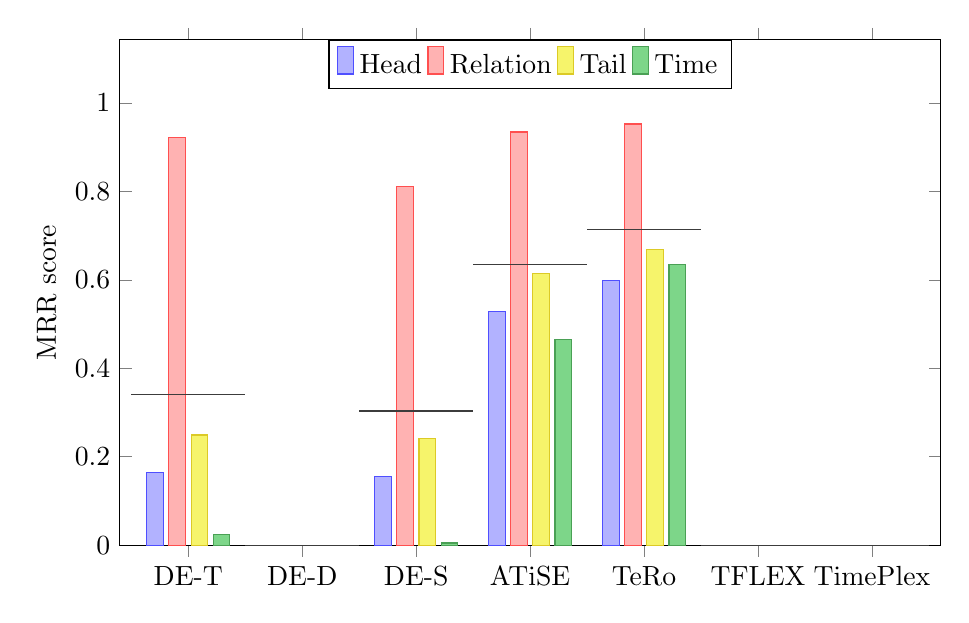
\begin{tikzpicture}
\begin{axis}[
    ybar,
    bar width=6pt,
    xticklabels={x,DE-T,DE-D,DE-S,ATiSE,TeRo,TFLEX,TimePlex},
    ymin=0,
    ymax=1.143125360701143,
    ylabel={MRR score},
    height=8cm,
    width=12cm,
    legend style={
        at={(0.5,1.0)},
        anchor=north,
        legend columns=-1
    },
    legend image code/.code={
        \draw [#1] (0cm,-0.1cm) rectangle (0.2cm,0.25cm); },
    ]
\addplot[color=ourdarkblue, fill=ourlightblue] coordinates { %head
(0, 0.1637073478821412) %DE_TransE
(1, 0) %DE_DistMult
(2, 0.15541381170193883) %DE_SimplE
(3, 0.5275712264361427) %ATISE
(4, 0.5983506476939411) %TERO
(5, 0) %TFLEX
(6, 0) %TimePlex
} ;
\addplot[color=ourdarkred, fill=ourlightred] coordinates { %relation
(0, 0.9230200501431489) %DE_TransE
(1, 0) %DE_DistMult
(2, 0.8116771918053982) %DE_SimplE
(3, 0.9345564000620602) %ATISE
(4, 0.9526044672509525) %TERO
(5, 0) %TFLEX
(6, 0) %TimePlex
} ;
\addplot[color=ourdarkyellow, fill=ourlightyellow] coordinates { %tail
(0, 0.24924584013892864) %DE_TransE
(1, 0) %DE_DistMult
(2, 0.2414293939480342) %DE_SimplE
(3, 0.6148980855055178) %ATISE
(4, 0.6696166224463463) %TERO
(5, 0) %TFLEX
(6, 0) %TimePlex
} ;
\addplot[color=ourdarkgreen, fill=ourlightgreen] coordinates { %time_from
(0, 0.024055630464001724) %DE_TransE
(1, 0) %DE_DistMult
(2, 0.0048056877918240416) %DE_SimplE
(3, 0.4657178150077794) %ATISE
(4, 0.6348767483602489) %TERO
(5, 0) %TFLEX
(6, 0) %TimePlex
} ;
\addplot[ourblack,sharp plot,update limits=false,] coordinates { %DE_TransE
(-0.5, 0.34000721715705284)
(0.5, 0.34000721715705284)
} ;
\addplot[ourblack,sharp plot,update limits=false,] coordinates { %DE_DistMult
(0.5, 0)
(1.5, 0)
} ;
\addplot[ourblack,sharp plot,update limits=false,] coordinates { %DE_SimplE
(1.5, 0.30333152131179775)
(2.5, 0.30333152131179775)
} ;
\addplot[ourblack,sharp plot,update limits=false,] coordinates { %ATISE
(2.5, 0.6356858817528941)
(3.5, 0.6356858817528941)
} ;
\addplot[ourblack,sharp plot,update limits=false,] coordinates { %TERO
(3.5, 0.7138621214378867)
(4.5, 0.7138621214378867)
} ;
\addplot[ourblack,sharp plot,update limits=false,] coordinates { %TFLEX
(4.5, 0)
(5.5, 0)
} ;
\addplot[ourblack,sharp plot,update limits=false,] coordinates { %TimePlex
(5.5, 0)
(6.5, 0)
} ;
\legend{Head,Relation,Tail,Time}
\end{axis}
\end{tikzpicture}
}
\caption{wikidata12k, split 2}
\label{fig:compare_wikidata12k_2}
\end{minipage}
\end{figure}

%\begin{figure}[htb]
\centering
\begin{minipage}{\columnwidthcaption}
\resizebox{\columnwidthcaption}{!}{
\centering
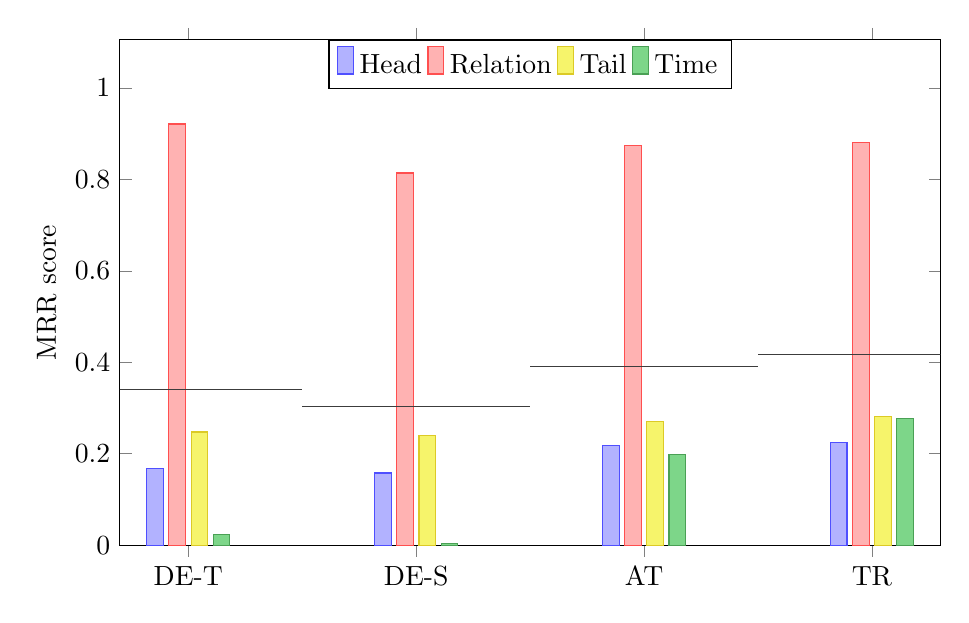
\begin{tikzpicture}
\begin{axis}[
    ybar,
    bar width=6pt,
    xtick={0,1,2,3},
    xticklabels={DE-T,DE-S,AT,TR},
    ymin=0,
    ymax=1.1055519622990757,
    ylabel={MRR score},
    height=8cm,
    width=12cm,
    legend style={
        at={(0.5,1.0)},
        anchor=north,
        legend columns=-1
    },
    legend image code/.code={
        \draw [#1] (0cm,-0.1cm) rectangle (0.2cm,0.25cm); },
    ]
\addplot[color=ourdarkblue, fill=ourlightblue] coordinates { %head
(0, 0.16856201354681669) %DE_TransE
(1, 0.1579443106395794) %DE_SimplE
(2, 0.21749963399555997) %ATISE
(3, 0.22541330553169855) %TERO
} ;
\addplot[color=ourdarkred, fill=ourlightred] coordinates { %relation
(0, 0.9212933019158965) %DE_TransE
(1, 0.8141468781135313) %DE_SimplE
(2, 0.8733535658464987) %ATISE
(3, 0.8817203020512926) %TERO
} ;
\addplot[color=ourdarkyellow, fill=ourlightyellow] coordinates { %tail
(0, 0.24762086236479688) %DE_TransE
(1, 0.24033615678654172) %DE_SimplE
(2, 0.2709493075129491) %ATISE
(3, 0.2820865071981324) %TERO
} ;
\addplot[color=ourdarkgreen, fill=ourlightgreen] coordinates { %time_from
(0, 0.023727251121544404) %DE_TransE
(1, 0.004434572351919235) %DE_SimplE
(2, 0.19870801166124544) %ATISE
(3, 0.2779541232922569) %TERO
} ;
\addplot[ourblack,sharp plot,update limits=false,] coordinates { %DE_TransE
(-0.5, 0.34030085723726033)
(0.5, 0.34030085723726033)
} ;
\addplot[ourblack,sharp plot,update limits=false,] coordinates { %DE_SimplE
(0.5, 0.30421547947288957)
(1.5, 0.30421547947288957)
} ;
\addplot[ourblack,sharp plot,update limits=false,] coordinates { %ATISE
(1.5, 0.3901276297540677)
(2.5, 0.3901276297540677)
} ;
\addplot[ourblack,sharp plot,update limits=false,] coordinates { %TERO
(2.5, 0.4167935595183541)
(3.5, 0.4167935595183541)
} ;
\legend{Head,Relation,Tail,Time}
\end{axis}
\end{tikzpicture}
}
\caption{WikiData, split 3}
\label{fig:compare_wikidata12k_3}
\end{minipage}
\end{figure}

%\clearpage
\begin{figure*}[ht]
\centering
\begin{minipage}{0.9\textwidth}
\centering
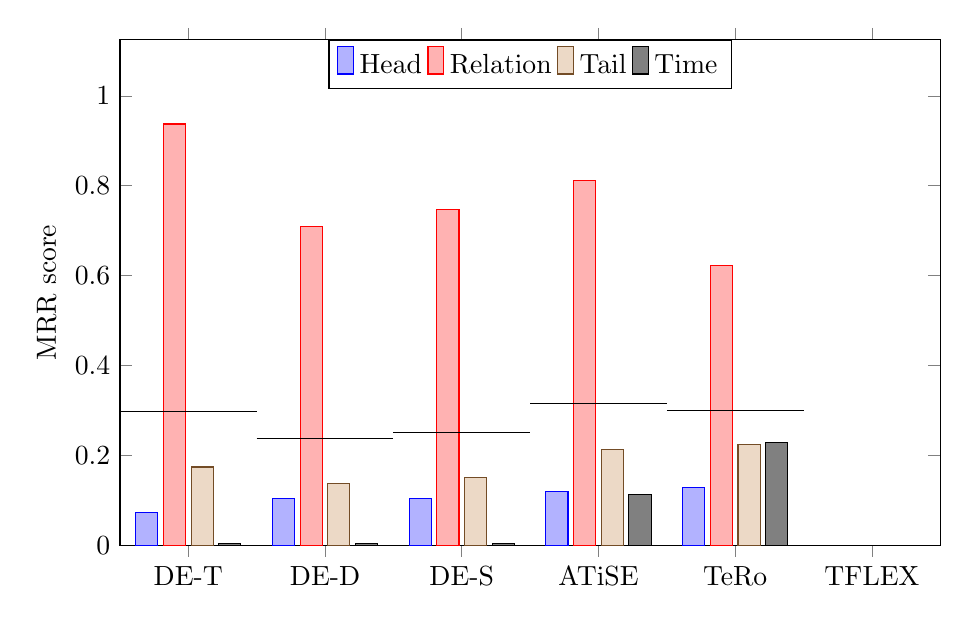
\begin{tikzpicture}
\begin{axis}[
    ybar,
    bar width=8pt,
    xticklabels={x,DE-T,DE-D,DE-S,ATiSE,TeRo,TFLEX},
    ymin=0,
    ymax=1.1248919226393623,
    ylabel={MRR score},
    height=8cm,
    width=12cm,
    legend style={
        at={(0.5,1.0)},
        anchor=north,
        legend columns=-1
    },
    legend image code/.code={
        \draw [#1] (0cm,-0.1cm) rectangle (0.2cm,0.25cm); },
    ]
\addplot coordinates { %head
(0, 0.07269008209368914) %DE_TransE
(1, 0.10403175627450587) %DE_DistMult
(2, 0.103908857857064) %DE_SimplE
(3, 0.11940060065365914) %ATISE
(4, 0.12810086873551824) %TERO
(5, 0) %TFLEX
} ;
\addplot coordinates { %relation
(0, 0.937409935532802) %DE_TransE
(1, 0.7083517138368421) %DE_DistMult
(2, 0.746826364220317) %DE_SimplE
(3, 0.8116911786950792) %ATISE
(4, 0.622934320897219) %TERO
(5, 0) %TFLEX
} ;
\addplot coordinates { %tail
(0, 0.1739083563401673) %DE_TransE
(1, 0.1364008382414642) %DE_DistMult
(2, 0.14965079657383037) %DE_SimplE
(3, 0.212866119662905) %ATISE
(4, 0.22319815155343745) %TERO
(5, 0) %TFLEX
} ;
\addplot coordinates { %time_from
(0, 0.004602542255970624) %DE_TransE
(1, 0.004026712387476274) %DE_DistMult
(2, 0.003965725310163026) %DE_SimplE
(3, 0.11365570730659119) %ATISE
(4, 0.22802233297323365) %TERO
(5, 0) %TFLEX
} ;
\addplot[black,sharp plot,update limits=false,] coordinates { %DE_TransE
(-0.5, 0.29715272905565693)
(0.5, 0.29715272905565693)
} ;
\addplot[black,sharp plot,update limits=false,] coordinates { %DE_DistMult
(0.5, 0.2382027551850705)
(1.5, 0.2382027551850705)
} ;
\addplot[black,sharp plot,update limits=false,] coordinates { %DE_SimplE
(1.5, 0.251087935990342)
(2.5, 0.251087935990342)
} ;
\addplot[black,sharp plot,update limits=false,] coordinates { %ATISE
(2.5, 0.3144034015795592)
(3.5, 0.3144034015795592)
} ;
\addplot[black,sharp plot,update limits=false,] coordinates { %TERO
(3.5, 0.30056391853985026)
(4.5, 0.30056391853985026)
} ;
\addplot[black,sharp plot,update limits=false,] coordinates { %TFLEX
(4.5, 0)
(5.5, 0)
} ;
\legend{Head,Relation,Tail,Time}
\end{axis}
\end{tikzpicture}
\caption{yago11k, split original}
\label{fig:compare_yago11k_original}
\end{minipage}
\end{figure*}

%\begin{figure*}[ht]
\centering
\begin{minipage}{0.9\textwidth}
\centering
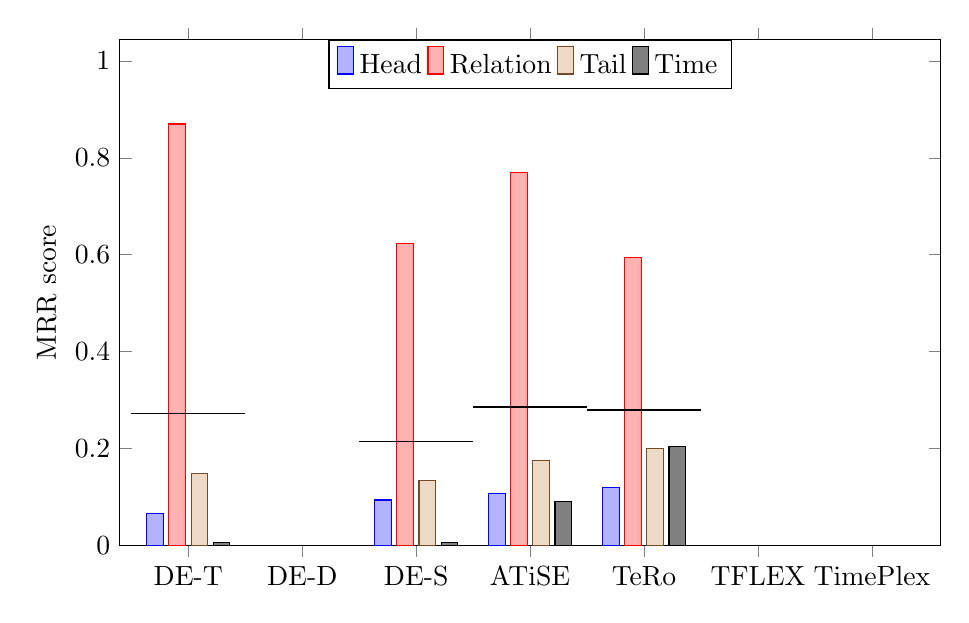
\begin{tikzpicture}
\begin{axis}[
    ybar,
    bar width=6pt,
    xticklabels={x,DE-T,DE-D,DE-S,ATiSE,TeRo,TFLEX,TimePlex},
    ymin=0,
    ymax=1.0437811938819743,
    ylabel={MRR score},
    height=8cm,
    width=12cm,
    legend style={
        at={(0.5,1.0)},
        anchor=north,
        legend columns=-1
    },
    legend image code/.code={
        \draw [#1] (0cm,-0.1cm) rectangle (0.2cm,0.25cm); },
    ]
\addplot coordinates { %head
(0, 0.0654146268614607) %DE_TransE
(1, 0) %DE_DistMult
(2, 0.09324680041983448) %DE_SimplE
(3, 0.10744684004886963) %ATISE
(4, 0.11929283069012821) %TERO
(5, 0) %TFLEX
(6, 0) %TimePlex
} ;
\addplot coordinates { %relation
(0, 0.869817661568312) %DE_TransE
(1, 0) %DE_DistMult
(2, 0.6224977810803526) %DE_SimplE
(3, 0.7688568564988466) %ATISE
(4, 0.5937145459898716) %TERO
(5, 0) %TFLEX
(6, 0) %TimePlex
} ;
\addplot coordinates { %tail
(0, 0.14793308392634577) %DE_TransE
(1, 0) %DE_DistMult
(2, 0.13363807469587557) %DE_SimplE
(3, 0.17418063844636406) %ATISE
(4, 0.1993527701241248) %TERO
(5, 0) %TFLEX
(6, 0) %TimePlex
} ;
\addplot coordinates { %time_from
(0, 0.005696572249049672) %DE_TransE
(1, 0) %DE_DistMult
(2, 0.004826684458969692) %DE_SimplE
(3, 0.09051857131363399) %ATISE
(4, 0.20448998452449743) %TERO
(5, 0) %TFLEX
(6, 0) %TimePlex
} ;
\addplot[black,sharp plot,update limits=false,] coordinates { %DE_TransE
(-0.5, 0.2722154861512923)
(0.5, 0.2722154861512923)
} ;
\addplot[black,sharp plot,update limits=false,] coordinates { %DE_DistMult
(0.5, 0)
(1.5, 0)
} ;
\addplot[black,sharp plot,update limits=false,] coordinates { %DE_SimplE
(1.5, 0.2135523351637587)
(2.5, 0.2135523351637587)
} ;
\addplot[black,sharp plot,update limits=false,] coordinates { %ATISE
(2.5, 0.2852507265769301)
(3.5, 0.2852507265769301)
} ;
\addplot[black,sharp plot,update limits=false,] coordinates { %TERO
(3.5, 0.2792125328321544)
(4.5, 0.2792125328321544)
} ;
\addplot[black,sharp plot,update limits=false,] coordinates { %TFLEX
(4.5, 0)
(5.5, 0)
} ;
\addplot[black,sharp plot,update limits=false,] coordinates { %TimePlex
(5.5, 0)
(6.5, 0)
} ;
\legend{Head,Relation,Tail,Time}
\end{axis}
\end{tikzpicture}
\caption{yago11k, split 1}
\label{fig:compare_yago11k_1}
\end{minipage}
\end{figure*}

%\begin{figure*}[ht]
\centering
\begin{minipage}{0.9\textwidth}
\centering
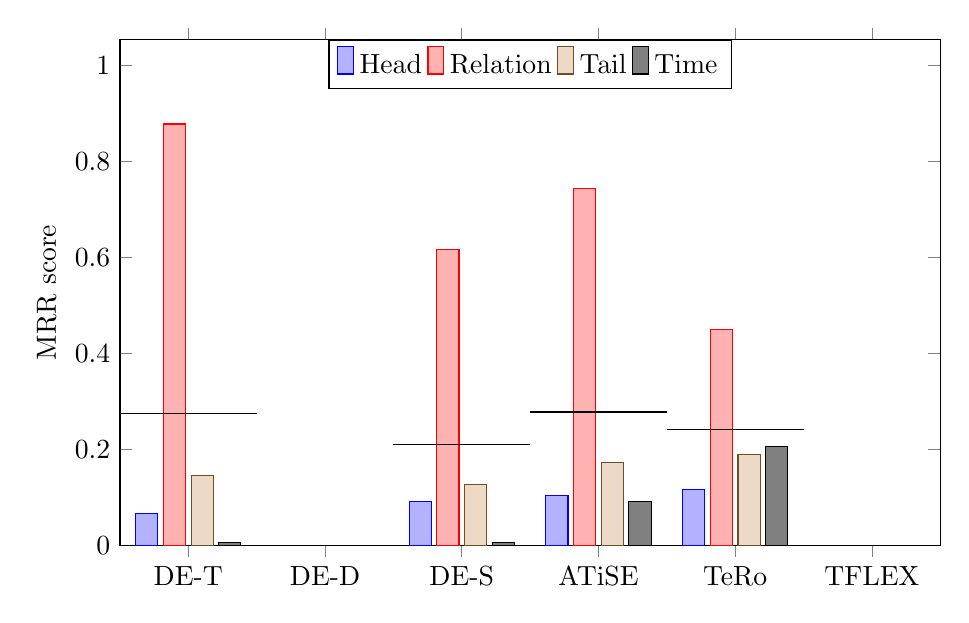
\begin{tikzpicture}
\begin{axis}[
    ybar,
    bar width=8pt,
    xticklabels={x,DE-T,DE-D,DE-S,ATiSE,TeRo,TFLEX},
    ymin=0,
    ymax=1.0537423369868102,
    ylabel={MRR score},
    height=8cm,
    width=12cm,
    legend style={
        at={(0.5,1.0)},
        anchor=north,
        legend columns=-1
    },
    legend image code/.code={
        \draw [#1] (0cm,-0.1cm) rectangle (0.2cm,0.25cm); },
    ]
\addplot coordinates { %head
(0, 0.06558515002873619) %DE_TransE
(1, 0) %DE_DistMult
(2, 0.09033631814543572) %DE_SimplE
(3, 0.1033600783877517) %ATISE
(4, 0.11618914859972021) %TERO
(5, 0) %TFLEX
} ;
\addplot coordinates { %relation
(0, 0.8781186141556753) %DE_TransE
(1, 0) %DE_DistMult
(2, 0.6167683241480337) %DE_SimplE
(3, 0.7438636467156967) %ATISE
(4, 0.4505377249751327) %TERO
(5, 0) %TFLEX
} ;
\addplot coordinates { %tail
(0, 0.14540485431774205) %DE_TransE
(1, 0) %DE_DistMult
(2, 0.12701248362579132) %DE_SimplE
(3, 0.17271991731482117) %ATISE
(4, 0.18895690258586312) %TERO
(5, 0) %TFLEX
} ;
\addplot coordinates { %time_from
(0, 0.006198447739629655) %DE_TransE
(1, 0) %DE_DistMult
(2, 0.005828410270192761) %DE_SimplE
(3, 0.09057026289935799) %ATISE
(4, 0.20601074153276433) %TERO
(5, 0) %TFLEX
} ;
\addplot[black,sharp plot,update limits=false,] coordinates { %DE_TransE
(-0.5, 0.2738267665604459)
(0.5, 0.2738267665604459)
} ;
\addplot[black,sharp plot,update limits=false,] coordinates { %DE_DistMult
(0.5, 0)
(1.5, 0)
} ;
\addplot[black,sharp plot,update limits=false,] coordinates { %DE_SimplE
(1.5, 0.20998638404736464)
(2.5, 0.20998638404736464)
} ;
\addplot[black,sharp plot,update limits=false,] coordinates { %ATISE
(2.5, 0.27762847632940946)
(3.5, 0.27762847632940946)
} ;
\addplot[black,sharp plot,update limits=false,] coordinates { %TERO
(3.5, 0.2404236294233677)
(4.5, 0.2404236294233677)
} ;
\addplot[black,sharp plot,update limits=false,] coordinates { %TFLEX
(4.5, 0)
(5.5, 0)
} ;
\legend{Head,Relation,Tail,Time}
\end{axis}
\end{tikzpicture}
\caption{yago11k, split 2}
\label{fig:compare_yago11k_2}
\end{minipage}
\end{figure*}

%\begin{figure*}[ht]
\centering
\begin{minipage}{0.9\textwidth}
\centering
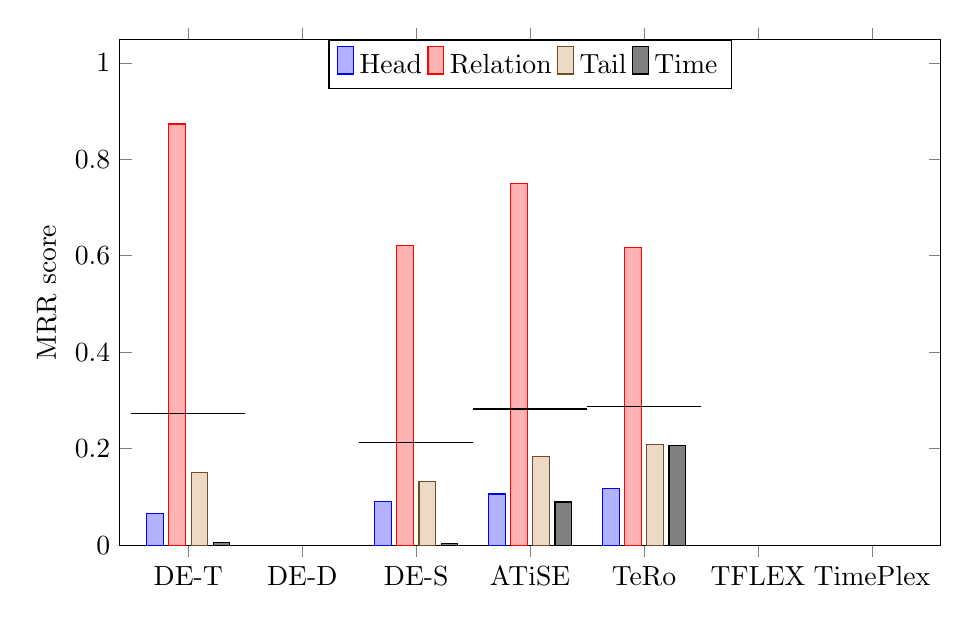
\begin{tikzpicture}
\begin{axis}[
    ybar,
    bar width=6pt,
    xticklabels={x,DE-T,DE-D,DE-S,ATiSE,TeRo,TFLEX,TimePlex},
    ymin=0,
    ymax=1.0478998699609892,
    ylabel={MRR score},
    height=8cm,
    width=12cm,
    legend style={
        at={(0.5,1.0)},
        anchor=north,
        legend columns=-1
    },
    legend image code/.code={
        \draw [#1] (0cm,-0.1cm) rectangle (0.2cm,0.25cm); },
    ]
\addplot coordinates { %head
(0, 0.06598500048947091) %DE_TransE
(1, 0) %DE_DistMult
(2, 0.0910450302298716) %DE_SimplE
(3, 0.10608125303624218) %ATISE
(4, 0.118174080416223) %TERO
(5, 0) %TFLEX
(6, 0) %TimePlex
} ;
\addplot coordinates { %relation
(0, 0.8732498916341577) %DE_TransE
(1, 0) %DE_DistMult
(2, 0.6221168235391219) %DE_SimplE
(3, 0.7494652308968521) %ATISE
(4, 0.6165239751613752) %TERO
(5, 0) %TFLEX
(6, 0) %TimePlex
} ;
\addplot coordinates { %tail
(0, 0.15003600005950565) %DE_TransE
(1, 0) %DE_DistMult
(2, 0.13284767704545358) %DE_SimplE
(3, 0.18365436889087297) %ATISE
(4, 0.2080882949555633) %TERO
(5, 0) %TFLEX
(6, 0) %TimePlex
} ;
\addplot coordinates { %time_from
(0, 0.005387766857512553) %DE_TransE
(1, 0) %DE_DistMult
(2, 0.00411020285253353) %DE_SimplE
(3, 0.08955133687896336) %ATISE
(4, 0.20698514239639496) %TERO
(5, 0) %TFLEX
(6, 0) %TimePlex
} ;
\addplot[black,sharp plot,update limits=false,] coordinates { %DE_TransE
(-0.5, 0.27366466476016243)
(0.5, 0.27366466476016243)
} ;
\addplot[black,sharp plot,update limits=false,] coordinates { %DE_DistMult
(0.5, 0)
(1.5, 0)
} ;
\addplot[black,sharp plot,update limits=false,] coordinates { %DE_SimplE
(1.5, 0.21252993341674445)
(2.5, 0.21252993341674445)
} ;
\addplot[black,sharp plot,update limits=false,] coordinates { %ATISE
(2.5, 0.28218804742573345)
(3.5, 0.28218804742573345)
} ;
\addplot[black,sharp plot,update limits=false,] coordinates { %TERO
(3.5, 0.2874428732323866)
(4.5, 0.2874428732323866)
} ;
\addplot[black,sharp plot,update limits=false,] coordinates { %TFLEX
(4.5, 0)
(5.5, 0)
} ;
\addplot[black,sharp plot,update limits=false,] coordinates { %TimePlex
(5.5, 0)
(6.5, 0)
} ;
\legend{Head,Relation,Tail,Time}
\end{axis}
\end{tikzpicture}
\caption{yago11k, split 3}
\label{fig:compare_yago11k_3}
\end{minipage}
\end{figure*}


\twocolumn

\end{document}
